% JIFMA manuscript — anonymous main document (double-blind: the cover page is a separate file). Journal of International Financial Management &
% Accounting, author information read 2026-11-10 (secondary copy; Wiley page not reachable by script): "Manuscripts generally should not exceed
% 30 pages in length (including endnotes, references, supporting exhibits and any appendices) ... double-spaced, except for indented quotations,
% endnotes and references ... abstract not to exceed 250 words ... authors should not identify themselves directly or indirectly".
% Tables and figures are placed after the reference list by endfloat (the reading copy built by the package script keeps them in place).
\documentclass[12pt]{article}
\usepackage[margin=1in]{geometry}\usepackage{mathptmx}\usepackage{setspace}\doublespacing
\usepackage{booktabs}\usepackage{array}\usepackage{amsmath}\usepackage{graphicx}\usepackage{threeparttable}\usepackage{rotating}
\newif\ifinlinefloats\inlinefloatstrue   % the package builder sets \inlinefloatstrue for the reading copy
\ifinlinefloats\else\usepackage[nolists,tablesfirst]{endfloat}\renewcommand{\efloatseparator}{\mbox{}}\DeclareDelayedFloatFlavor{sidewaystable}{table}\fi
\usepackage[hidelinks]{hyperref}\usepackage{url}\usepackage{apacite}
% generated by code/make_tables_jifma.py on 2026-11-11 (inherits make_tables_cgir.py) — every macro traces to a results file (see the generators for keys)
\newcommand{\NOldN}{464}
\newcommand{\NOldDisposed}{257}
\newcommand{\NOldRetained}{89}
\newcommand{\NOldOther}{43}
\newcommand{\NOldUnresolved}{75}
\newcommand{\NOldPriced}{380}
\newcommand{\NOldPricedOneY}{366}
\newcommand{\NOldOwnership}{387}
\newcommand{\NNewN}{294}
\newcommand{\NNewDisposed}{145}
\newcommand{\NNewRetained}{90}
\newcommand{\NNewOther}{29}
\newcommand{\NNewUnresolved}{30}
\newcommand{\NNewPriced}{260}
\newcommand{\NNewPricedOneY}{249}
\newcommand{\NNewOwnership}{283}
\newcommand{\NAllN}{758}
\newcommand{\NAllDisposed}{402}
\newcommand{\NAllRetained}{179}
\newcommand{\NAllOther}{72}
\newcommand{\NAllUnresolved}{105}
\newcommand{\NAllPriced}{640}
\newcommand{\NAllPricedOneY}{615}
\newcommand{\NAllOwnership}{670}
\newcommand{\NScoreOneY}{559}
\newcommand{\NLabelOneY}{471}
\newcommand{\NGateOne}{579}
\newcommand{\AUCPooledLLM}{0.761}
\newcommand{\AUCPooledFin}{0.587}
\newcommand{\AUCNewLLM}{0.813}
\newcommand{\AUCNewFin}{0.577}
\newcommand{\DeltaPooled}{0.174}
\newcommand{\DeltaPooledLo}{0.117}
\newcommand{\DeltaPooledHi}{0.235}
\newcommand{\AUCOldIdent}{0.706}
\newcommand{\AUCOldAnon}{0.691}
\newcommand{\AUCNewIdent}{0.810}
\newcommand{\AUCNewAnon}{0.803}
\newcommand{\ClaudeOutsideKnowledgeOld}{43.0}
\newcommand{\AUCClaudeFlaggedAnonOld}{0.763}
\newcommand{\AUCClaudeFlaggedIdentOld}{0.764}
\newcommand{\DisposedSharePooled}{69.3}
\newcommand{\GapOldLo}{$-$0.006}
\newcommand{\GapOldHi}{0.039}
\newcommand{\AUCEarlyPooled}{0.780}
\newcommand{\AUCEarlyNew}{0.919}
\newcommand{\AUCEarlyOld}{0.698}
\newcommand{\AUCLateVsNever}{0.708}
\newcommand{\SpearmanAnon}{$-$0.135}
\newcommand{\NAUCEarlyAnon}{339}
\newcommand{\NAUCEarly}{412}
\newcommand{\SpearmanAnonP}{0.001}
\newcommand{\RankAnonCoef}{$-$0.195}
\newcommand{\RankAnonP}{0.005}
\newcommand{\AUCEarlyAnon}{0.817}
\newcommand{\QQDiff}{$-$4.4}
\newcommand{\QQLo}{$-$22.7}
\newcommand{\QQHi}{+17.3}
\newcommand{\QQWithinYear}{$-$11.7}
\newcommand{\QQWithinYearP}{0.154}
\newcommand{\SpearmanScoreBhar}{$-$0.136}
\newcommand{\SpearmanScoreBharP}{0.001}
\newcommand{\SpearmanWithinYear}{$-$0.134}
\newcommand{\SpearmanWithinYearP}{0.002}
\newcommand{\AnnCarSlope}{0.037}
\newcommand{\AnnCarSlopeSE}{0.019}
\newcommand{\AnnCarSlopeP}{0.046}
\newcommand{\CTHiLo}{$-$12.2}
\newcommand{\CTHiLoT}{$-$1.68}
\newcommand{\FFHiLo}{$-$0.52}
\newcommand{\FFHiLoT}{$-$0.96}
\newcommand{\DriftMean}{$-$6.0}
\newcommand{\DriftMedian}{$-$15.9}
\newcommand{\DriftNeg}{66}
\newcommand{\DriftLo}{$-$11.6}
\newcommand{\DriftHi}{$-$0.1}
\newcommand{\AnnCarMean}{+0.58}
\newcommand{\AnnCarT}{1.30}
\newcommand{\AnnCarN}{583}
\newcommand{\FFAllAlpha}{$-$0.02}
\newcommand{\FFAllT}{$-$0.07}
\newcommand{\EarlyN}{195}
\newcommand{\EarlyMean}{$-$14.2}
\newcommand{\EarlyMedian}{$-$26.6}
\newcommand{\NeverN}{141}
\newcommand{\NeverMean}{+1.4}
\newcommand{\NeverMedian}{$-$8.7}
\newcommand{\EarlyNeverDiff}{$-$15.6}
\newcommand{\EarlyNeverLo}{$-$34.2}
\newcommand{\EarlyNeverHi}{+1.3}
\newcommand{\EarlyNeverWelchP}{0.082}
\newcommand{\EarlyNeverMWP}{0.001}
\newcommand{\LateMean}{$-$3.8}
\newcommand{\LateNeverP}{0.626}
\newcommand{\DispRetDiff}{$-$10.3}
\newcommand{\DispRetMWP}{0.010}
\newcommand{\DispRetWelchP}{0.219}
\newcommand{\RankSpecOneCoef}{$-$0.191}
\newcommand{\RankSpecOneP}{0.004}
\newcommand{\RankSpecOneClP}{0.001}
\newcommand{\RankSpecTwoCoef}{$-$0.192}
\newcommand{\RankSpecTwoP}{0.003}
\newcommand{\RankSpecTwoClP}{$<$0.001}
\newcommand{\RankSpecThreeCoef}{$-$0.195}
\newcommand{\RankSpecThreeP}{0.004}
\newcommand{\RankSpecThreeClP}{$<$0.001}
\newcommand{\RankSpecThreeBCoef}{$-$0.229}
\newcommand{\RankSpecThreeBP}{0.019}
\newcommand{\RankSpecThreeBClP}{0.002}
\newcommand{\RankSpecThreeCCoef}{$-$0.168}
\newcommand{\RankSpecThreeCP}{0.097}
\newcommand{\RankSpecThreeCClP}{0.047}
\newcommand{\RankSpecFourCoef}{$-$0.207}
\newcommand{\RankSpecFourP}{0.047}
\newcommand{\RankSpecFourClP}{0.042}
\newcommand{\RankScoreCoefMin}{$-$0.20}
\newcommand{\RankScoreCoefMax}{$-$0.19}
\newcommand{\JointEarlyCoef}{$-$0.151}
\newcommand{\JointEarlyP}{0.083}
\newcommand{\JointScoreCoef}{0.135}
\newcommand{\JointScoreP}{0.549}
\newcommand{\BlockMedian}{34.6}
\newcommand{\LargestMedian}{21.8}
\newcommand{\NOwnership}{551}
\newcommand{\ScoreOnBlock}{$-$0.113}
\newcommand{\ScoreOnBlockP}{0.013}
\newcommand{\ScoreOnBlockClP}{0.004}
\newcommand{\LowBlockDisp}{74}
\newcommand{\HighBlockDisp}{62}
\newcommand{\LowBlockEarly}{52}
\newcommand{\HighBlockEarly}{43}
\newcommand{\LowBlockMedian}{$-$26.9}
\newcommand{\HighBlockMedian}{$-$9.1}
\newcommand{\LowBlockMean}{$-$13.7}
\newcommand{\HighBlockMean}{$-$0.5}
\newcommand{\LowHighMWP}{$<$0.001}
\newcommand{\LowHighDiff}{$-$13.1}
\newcommand{\LowBlockMax}{27}
\newcommand{\HighBlockMin}{43}
\newcommand{\RankOnBlock}{0.14}
\newcommand{\RankOnBlockP}{0.062}
\newcommand{\ProtectPre}{0.5}
\newcommand{\ProtectPost}{95.5}
\newcommand{\ListingPre}{9.1}
\newcommand{\ListingPost}{77.3}
\newcommand{\CarPre}{+0.06}
\newcommand{\CarPost}{+5.29}
\newcommand{\CarPrePostP}{$<$0.001}
\newcommand{\ScorePre}{0.528}
\newcommand{\ScorePost}{0.510}
\newcommand{\ScorePrePostP}{0.616}
\newcommand{\EarlyPre}{40.2}
\newcommand{\NPostOutcomes}{19}
\newcommand{\EarlyPost}{36.8}
\newcommand{\EarlyPrePostP}{1.000}
\newcommand{\NPost}{49}
\newcommand{\NPostFilings}{44}
\newcommand{\FilingsPerYearPre}{39.0}
\newcommand{\FilingsPerYearPost}{16.4}
\newcommand{\NDefs}{10}
\newcommand{\IPOShare}{3.3}
\newcommand{\NClean}{581}
\newcommand{\KLAnnCar}{0.853}
\newcommand{\KLBhar}{$-$10.995}
\newcommand{\KLCar}{$-$7.857}
\newcommand{\KLDisposed}{69.3}
\newcommand{\KLN}{525}
\newcommand{\KLOwnMedian}{14.71}
\newcommand{\KLOwnMean}{18.432}
\newcommand{\RepeatCorrA}{0.96}
\newcommand{\RepeatCorrB}{0.99}
\newcommand{\BetweenModelCorr}{0.87}
\newcommand{\NRepeat}{245}
\newcommand{\KRXCompustatCorr}{0.9998}
\newcommand{\NPriceOverlap}{233}
\newcommand{\GlitchExcluded}{14}
\newcommand{\OwnPairs}{357}
\newcommand{\OwnWithinOne}{354}
\newcommand{\OwnDisagree}{3}
\newcommand{\AUCTemporalFin}{0.611}
\newcommand{\AUCTemporalLLM}{0.813}
\newcommand{\AnnCarSlopePP}{3.7}
\newcommand{\RankSpecThreePctl}{19.5}
\newcommand{\GPTOutsideKnowledgeOld}{3.8}
\newcommand{\CleanDisposedShare}{69.2}
\newcommand{\KLListed}{4.0}
\newcommand{\BlockOnDisposed}{$-$0.092}
\newcommand{\BlockOnDisposedSE}{0.129}
\newcommand{\BlockOnEarlyAlone}{$-$0.141}
\newcommand{\BlockOnEarlyAloneSE}{0.144}
\newcommand{\BlockOnEarlyWithScore}{0.113}
\newcommand{\BlockOnEarlyWithScoreSE}{0.133}
\newcommand{\ScoreOnEarlyWithBlock}{1.235}
\newcommand{\BlockOnCar}{0.030}
\newcommand{\BlockOnCarSE}{0.023}
\newcommand{\EarlyCoefBhar}{$-$0.243}
\newcommand{\LowBlockCoefBhar}{$-$0.231}
\newcommand{\InterCoefBhar}{0.223}
\newcommand{\InterPBhar}{0.114}
\newcommand{\EarlyCoefRank}{$-$0.136}
\newcommand{\LowBlockCoefRank}{$-$0.111}
\newcommand{\InterCoefRank}{0.114}
\newcommand{\InterPRank}{0.071}
\newcommand{\EarlyInLowBlockRank}{$-$0.022}
\newcommand{\LGScore}{0.76}
\newcommand{\LGAnnCar}{$-$7.3}
\newcommand{\LGBhar}{$-$15.3}
\newcommand{\KLKrxTotal}{948}
\newcommand{\KLKrxCaptive}{719}
\newcommand{\NScored}{720}
\newcommand{\QOneMedian}{$-$3.0}
\newcommand{\QFiveMedian}{$-$23.0}
\newcommand{\QQMedianDiff}{$-$20.0}
\newcommand{\QQMWP}{0.008}
\newcommand{\KLLGDrop}{30}
\newcommand{\NSensitive}{11}
\newcommand{\NMixed}{4}
\newcommand{\ExDoosanScore}{0.98}
\newcommand{\ExDoosanOutcome}{disposed}
\newcommand{\ExDBScore}{0.24}
\newcommand{\ExDBOutcome}{retained}
\newcommand{\ExTvingScore}{0.85}
\newcommand{\ExTvingOutcome}{disposed}
\newcommand{\NUnread}{38}
\newcommand{\NUnreadTooRecent}{15}
\newcommand{\NUnreadUnmatched}{13}
\newcommand{\NUnreadMergedLiq}{9}
\newcommand{\NUnreadClean}{1}
\newcommand{\NPostAll}{66}
\newcommand{\KLBharOne}{$-$11.0}
\newcommand{\KLOwnMeanOne}{18.4}
\newcommand{\KLOwnMedianOne}{14.7}
\newcommand{\MDEEarlyPP}{34}
\newcommand{\MDEScore}{0.10}
\newcommand{\ScoreSDPre}{0.22}
\newcommand{\NestedMZero}{0.587}
\newcommand{\NestedMZeroOld}{0.445}
\newcommand{\NestedMZeroNew}{0.581}
\newcommand{\NestedMOne}{0.667}
\newcommand{\NestedMOneOld}{0.566}
\newcommand{\NestedMOneNew}{0.668}
\newcommand{\NestedMTwo}{0.680}
\newcommand{\NestedMTwoOld}{0.599}
\newcommand{\NestedMTwoNew}{0.733}
\newcommand{\NestedMThree}{0.770}
\newcommand{\NestedMThreeOld}{0.706}
\newcommand{\NestedMThreeNew}{0.830}
\newcommand{\NestedF}{0.611}
\newcommand{\NestedFOld}{0.593}
\newcommand{\NestedFNew}{0.689}
\newcommand{\NestedKOne}{0.590}
\newcommand{\NestedKOneOld}{0.521}
\newcommand{\NestedKOneNew}{0.600}
\newcommand{\NestedS}{0.758}
\newcommand{\NestedSOld}{0.700}
\newcommand{\NestedSNew}{0.809}
\newcommand{\NestedIncMThreeMTwo}{+0.09}
\newcommand{\NestedIncMThreeMTwoLo}{0.05}
\newcommand{\NestedIncMThreeMTwoHi}{0.13}
\newcommand{\NestedIncMOneMZero}{+0.08}
\newcommand{\NestedIncKOneMZero}{+0.003}
\newcommand{\NestedIncMThreeMZero}{+0.18}
\newcommand{\NestedLRpMThree}{$<$0.001}
\newcommand{\DecompRTwo}{0.44}
\newcommand{\DecompAUCFitted}{0.675}
\newcommand{\DecompAUCResid}{0.722}
\newcommand{\DecompSaleCoef}{0.32}
\newcommand{\DecompFundCoef}{0.08}
\newcommand{\DecompInvestorCoef}{0.042}
\newcommand{\RankSPlusPurpose}{$-$0.285}
\newcommand{\RankSPlusPurposeP}{0.001}
\newcommand{\RankSPlusPurposeMentions}{$-$0.296}
\newcommand{\RankSPlusPurposeMentionsP}{$<$0.001}
\newcommand{\AnnSPlusPurposeMentions}{0.037}
\newcommand{\AnnSPlusPurposeMentionsP}{0.121}
\newcommand{\PermAUCMin}{0.48}
\newcommand{\PermAUCMax}{0.51}
\newcommand{\CoxN}{484}
\newcommand{\CoxEvents}{324}
\newcommand{\CoxConcordance}{0.73}
\newcommand{\CoxHRSD}{1.96}
\newcommand{\CoxHRSDLo}{1.74}
\newcommand{\CoxHRSDHi}{2.19}
\newcommand{\CoxHRUnit}{36.7}
\newcommand{\CoxHRBlock}{0.964}
\newcommand{\CoxHRBlockLo}{0.908}
\newcommand{\CoxHRBlockHi}{1.024}
\newcommand{\KMLowOneY}{24}
\newcommand{\KMMidOneY}{54}
\newcommand{\KMHighOneY}{74}
\newcommand{\KMAllOneY}{51}
\newcommand{\KMAllFiveY}{68}
\newcommand{\CoxPermHR}{1.22}
\newcommand{\CoxPHp}{0.054}
\newcommand{\RankSSector}{$-$0.194}
\newcommand{\RankSSectorPFirm}{0.004}
\newcommand{\RankSSectorPTwoway}{$<$0.001}
\newcommand{\RankSSic}{$-$0.153}
\newcommand{\RankSGind}{$-$0.167}
\newcommand{\RankSForeign}{$-$0.211}
\newcommand{\RankSForeignP}{0.002}
\newcommand{\RankSForeignN}{540}
\newcommand{\RankSBoard}{$-$0.187}
\newcommand{\RankSBoardP}{0.119}
\newcommand{\RankSBoardN}{194}
\newcommand{\AnnSSector}{0.045}
\newcommand{\AnnSSectorP}{0.020}
\newcommand{\ForeignCoverage}{577}
\newcommand{\ForeignMedian}{2.5}
\newcommand{\BoardN}{211}
\newcommand{\BoardMedian}{0.25}
\newcommand{\EarlySector}{$-$0.077}
\newcommand{\EarlySectorP}{0.013}
\newcommand{\BenchMarketAdjustedPaperRank}{$-$0.195}
\newcommand{\BenchMarketAdjustedPaperRankP}{0.004}
\newcommand{\BenchMarketAdjustedPaperMean}{$-$5.6}
\newcommand{\BenchMarketAdjustedPaperRho}{$-$0.137}
\newcommand{\BenchMarketAdjustedPaperN}{559}
\newcommand{\BenchPfSizebmWithSizeFallbackRank}{$-$0.147}
\newcommand{\BenchPfSizebmWithSizeFallbackRankP}{0.031}
\newcommand{\BenchPfSizebmWithSizeFallbackMean}{$-$8.2}
\newcommand{\BenchPfSizebmWithSizeFallbackRho}{$-$0.090}
\newcommand{\BenchPfSizebmWithSizeFallbackN}{540}
\newcommand{\BenchPfStrictRank}{$-$0.117}
\newcommand{\BenchPfStrictRankP}{0.095}
\newcommand{\BenchPfStrictMean}{$-$7.7}
\newcommand{\BenchPfStrictRho}{$-$0.073}
\newcommand{\BenchPfStrictN}{513}
\newcommand{\BenchPfRank}{$-$0.164}
\newcommand{\BenchPfRankP}{0.019}
\newcommand{\BenchPfMean}{$-$8.1}
\newcommand{\BenchPfRho}{$-$0.085}
\newcommand{\BenchPfN}{513}
\newcommand{\BenchMatchedFirmSizebmRank}{$-$0.017}
\newcommand{\BenchMatchedFirmSizebmRankP}{0.820}
\newcommand{\BenchMatchedFirmSizebmMean}{$-$8.6}
\newcommand{\BenchMatchedFirmSizebmRho}{$-$0.026}
\newcommand{\BenchMatchedFirmSizebmN}{504}
\newcommand{\BenchPsmControlFirmRank}{$-$0.124}
\newcommand{\BenchPsmControlFirmRankP}{0.071}
\newcommand{\BenchPsmControlFirmMean}{$-$3.6}
\newcommand{\BenchPsmControlFirmRho}{$-$0.088}
\newcommand{\BenchPsmControlFirmN}{522}
\newcommand{\SelFirmYears}{43,000}
\newcommand{\SelEvents}{615}
\newcommand{\SelFirms}{3,132}
\newcommand{\SelPseudoR}{0.061}
\newcommand{\SelLogAt}{0.231}
\newcommand{\SelLogAtP}{$<$0.001}
\newcommand{\SelLev}{0.627}
\newcommand{\SelLevP}{0.010}
\newcommand{\SelCf}{$-$2.963}
\newcommand{\SelCfP}{$<$0.001}
\newcommand{\SelSg}{0.186}
\newcommand{\SelSgP}{0.002}
\newcommand{\SelKosdaq}{$-$0.067}
\newcommand{\SelKosdaqP}{0.551}
\newcommand{\SelQ}{0.065}
\newcommand{\SelQP}{0.125}
\newcommand{\SelInv}{0.423}
\newcommand{\SelInvP}{0.609}
\newcommand{\SelCash}{$-$0.344}
\newcommand{\SelCashP}{0.324}
\newcommand{\SelPSAUC}{0.72}
\newcommand{\SelSupport}{100}
\newcommand{\BlockScoreSector}{$-$0.095}
\newcommand{\BlockScoreSectorP}{0.041}
\newcommand{\BlockScoreForeign}{$-$0.143}
\newcommand{\BlockScoreForeignP}{0.002}
\newcommand{\BlockScoreBoard}{$-$0.217}
\newcommand{\BlockScoreBoardP}{0.018}
\newcommand{\BlockScoreBoardN}{191}
\newcommand{\ForeignOnScore}{$-$0.222}
\newcommand{\ForeignOnScoreP}{0.016}
\newcommand{\DiDCxP}{5.45}
\newcommand{\DiDCxPSE}{1.59}
\newcommand{\DiDCxPP}{0.001}
\newcommand{\DiDN}{279}
\newcommand{\DiDNCaptive}{230}
\newcommand{\DiDNEquity}{49}
\newcommand{\DiDNPost}{65}
\newcommand{\DiDCxPLong}{6.52}
\newcommand{\DiDCxPLongP}{$<$0.001}
\newcommand{\DiDPlacebo}{2.27}
\newcommand{\DiDPlaceboP}{0.435}
\newcommand{\DiDCxPTwentyOne}{2.11}
\newcommand{\DiDCxPTwentyOneP}{0.661}
\newcommand{\CarCaptivePre}{$-$0.09}
\newcommand{\CarCaptivePost}{5.51}
\newcommand{\CarEquityPre}{$-$0.28}
\newcommand{\CarEquityPost}{$-$1.30}
\newcommand{\NEquityPost}{24}
\newcommand{\NCaptivePost}{51}
\newcommand{\AppraisalPrices}{40}
\newcommand{\AppraisalProxyDiff}{0.8}
\newcommand{\MoneynessMedian}{1.6}
\newcommand{\MoneynessITM}{60}
\newcommand{\MoneynessQOne}{$-$4.0}
\newcommand{\MoneynessQThree}{4.5}
\newcommand{\PutSlopeTwentyOne}{0.45}
\newcommand{\PutSlopeTwentyOneP}{0.015}
\newcommand{\PutSlopeTwentyOneN}{25}
\newcommand{\PutSlopeThree}{0.39}
\newcommand{\PutSlopeThreeP}{0.172}
\newcommand{\PutSlopeThreeN}{33}
\newcommand{\PutPlaceboPre}{$-$0.074}
\newcommand{\PutPlaceboPreP}{0.072}
\newcommand{\ExerciseMinusHold}{1.1}
\newcommand{\ExerciseBeats}{51}
\newcommand{\ExerciseN}{35}
\newcommand{\ProtPostWithBlock}{61}
\newcommand{\ProtPostN}{66}
\newcommand{\ProtPreWithBlock}{0}
\newcommand{\ProtPreN}{228}
\newcommand{\ProtCharterVote}{7}
\newcommand{\ProtNoListingHorizon}{3}
\newcommand{\ProtSalePlan}{4}
\newcommand{\ProtUnlistedSoft}{32}
\newcommand{\ProtNone}{15}
\newcommand{\ProtStrengthRho}{$-$0.27}
\newcommand{\ProtStrengthP}{0.075}
\newcommand{\ProtDisposedStrengthZero}{62}
\newcommand{\ProtDisposedStrengthOne}{17}
\newcommand{\ProtNLabStrengthZero}{13}
\newcommand{\ProtNLabStrengthOne}{23}
\newcommand{\ProtMeanSNone}{0.68}
\newcommand{\ProtMeanSCharter}{0.50}
\newcommand{\ProtMeanSUnlisted}{0.45}
\newcommand{\ProtMeanSHorizon}{0.34}
\newcommand{\ValN}{579}
\newcommand{\ValAUCId}{0.758}
\newcommand{\ValAUCAn}{0.751}
\newcommand{\ValDAUC}{0.007}
\newcommand{\ValDAUCLo}{$-$0.007}
\newcommand{\ValDAUCHi}{0.021}
\newcommand{\ValDAUCMaxSub}{0.022}
\newcommand{\ValOutsideA}{42}
\newcommand{\ValOutsideB}{4}
\newcommand{\ValSubsetN}{239}
\newcommand{\ValSubsetAUCId}{0.784}
\newcommand{\ValSubsetAUCAn}{0.780}
\newcommand{\ValSubsetDAUC}{0.003}
\newcommand{\ValSubsetLo}{$-$0.035}
\newcommand{\ValSubsetHi}{0.038}
\newcommand{\ValAUCPeriodEarly}{0.64}
\newcommand{\ValGapPeriodEarly}{$-$0.23}
\newcommand{\ValAUCPeriodMiddle}{0.75}
\newcommand{\ValGapPeriodMiddle}{$-$0.22}
\newcommand{\ValAUCPeriodLate}{0.81}
\newcommand{\ValGapPeriodLate}{$-$0.10}
\newcommand{\ValLRDiscPeriod}{0.425}
\newcommand{\ValLRCalPeriod}{0.010}
\newcommand{\ValAUCListedListed}{0.79}
\newcommand{\ValGapListedListed}{$-$0.17}
\newcommand{\ValAUCListedUnlisted}{0.66}
\newcommand{\ValGapListedUnlisted}{$-$0.18}
\newcommand{\ValLRDiscListed}{0.015}
\newcommand{\ValLRCalListed}{0.660}
\newcommand{\ValAUCKosdaqKosdaq}{0.77}
\newcommand{\ValGapKosdaqKosdaq}{$-$0.23}
\newcommand{\ValAUCKosdaqKospiOther}{0.76}
\newcommand{\ValGapKosdaqKospiOther}{$-$0.14}
\newcommand{\ValLRDiscKosdaq}{0.218}
\newcommand{\ValLRCalKosdaq}{0.060}
\newcommand{\ValAUCSizeLarge}{0.82}
\newcommand{\ValGapSizeLarge}{$-$0.03}
\newcommand{\ValAUCSizeMid}{0.85}
\newcommand{\ValGapSizeMid}{$-$0.06}
\newcommand{\ValAUCSizeSmall}{0.63}
\newcommand{\ValGapSizeSmall}{$-$0.27}
\newcommand{\ValLRDiscSize}{0.026}
\newcommand{\ValLRCalSize}{$<$0.001}
\newcommand{\ValAUCMcapLarge}{0.82}
\newcommand{\ValGapMcapLarge}{$-$0.06}
\newcommand{\ValAUCMcapMid}{0.75}
\newcommand{\ValGapMcapMid}{$-$0.17}
\newcommand{\ValAUCMcapSmall}{0.76}
\newcommand{\ValGapMcapSmall}{$-$0.29}
\newcommand{\ValLRDiscMcap}{0.514}
\newcommand{\ValLRCalMcap}{$<$0.001}
\newcommand{\ValAUCForeignHigh}{0.83}
\newcommand{\ValGapForeignHigh}{$-$0.11}
\newcommand{\ValAUCForeignLow}{0.64}
\newcommand{\ValGapForeignLow}{$-$0.24}
\newcommand{\ValAUCForeignMid}{0.79}
\newcommand{\ValGapForeignMid}{$-$0.17}
\newcommand{\ValLRDiscForeign}{0.245}
\newcommand{\ValLRCalForeign}{0.198}
\newcommand{\ValMeanS}{0.52}
\newcommand{\ValMeanY}{0.69}
\newcommand{\ValRecalSlope}{1.46}
\newcommand{\ValStageOneRTwo}{0.53}
\newcommand{\ValMaxBeta}{0.19}
\newcommand{\ValErrSizeBeta}{+0.15}
\newcommand{\ValErrSizeP}{0.005}
\newcommand{\KappaSale}{0.90}
\newcommand{\KappaFund}{0.92}
\newcommand{\KappaHolding}{0.84}
\newcommand{\KappaEff}{0.84}
\newcommand{\KappaBuyer}{0.82}
\newcommand{\KappaAppraisal}{0.76}
\newcommand{\KappaListing}{0.01}
\newcommand{\KappaProtect}{0.24}
\newcommand{\KappaInvestor}{0.46}
\newcommand{\TwoModelCorr}{0.80}
\newcommand{\TwoModelCorrNew}{0.87}
\newcommand{\TwoModelN}{715}
\newcommand{\TwoModelMeanA}{0.59}
\newcommand{\TwoModelMeanB}{0.46}
\newcommand{\WithinModelMinAgree}{0.86}
\newcommand{\KLSale}{12.0}
\newcommand{\KLRetained}{30.7}
\newcommand{\KLSpecial}{89.1}
\newcommand{\KLEff}{5.9}
\newcommand{\OurSaleStrict}{8.5}
\newcommand{\OurSaleBroad}{22.4}
\newcommand{\OurSpecial}{99}
\newcommand{\OurEff}{97}
\newcommand{\OurKLN}{517}
\newcommand{\OurListedShare}{3.9}
\newcommand{\OurRetainedShare}{26.0}
\newcommand{\OurRetainedUpper}{40.3}
\newcommand{\OurOutcomeN}{412}
\newcommand{\RepeatAbsA}{0.04}
\newcommand{\RepeatAbsB}{0.02}
\newcommand{\LabelCrossAgree}{74/85}
\newcommand{\LabelCrossPct}{87.1}
\newcommand{\IndustryParents}{459}
\newcommand{\IndustryEvents}{576}

\newif\ifanon\anontrue   % the package builder sets \anonfalse for the author copy
% filled 2026-11-14 from the Zenodo record of release v2.1-jifma (concept DOI unchanged); verified through the public API (records/24220450) and doi.org (302)
\newcommand{\ArchiveTag}{v2.1-jifma}
\newcommand{\ArchiveVersionDOI}{10.5281/zenodo.24220450}
\newcommand{\ArchiveConceptDOI}{10.5281/zenodo.23660635}
       % \ArchiveTag, \ArchiveVersionDOI, \ArchiveConceptDOI
\newcommand{\tabnote}[1]{\par\vspace{4pt}\begin{minipage}{\linewidth}\singlespacing\small\emph{Note.} #1\end{minipage}}
\newcommand{\captive}{captive spin-off}
\title{Controlling Owners, Disclosed Intentions, and Minority Shareholder Returns in Korean Captive Spin-Offs}
\author{}\date{}
\begin{document}
\maketitle
\thispagestyle{empty}
\subsection*{Abstract}
\noindent In a Korean \captive{} a listed parent moves a business into a wholly owned subsidiary; whether it is later kept, sold or listed is decided by the controlling owner without a shareholder vote, and any loss to the minority comes at the disposal. The literature on controlling-owner expropriation infers intention from the expropriating outcome; we measure beforehand what the filing disclosed about the risk that the subsidiary would not be kept. Two language models read the division filings of \NScored{} \captive{}s of 2001--2026 and forecast whether the parent will still own the subsidiary three to five years later. For the \NGateOne{} labelled divisions the forecast predicts the realised disposal (AUC \AUCPooledLLM{}) beyond the filing's financials and the purpose categories and mention flags a hand coder would record, survives the removal of every name and date, and doubles the hazard of disposal per standard deviation. The announcement return rises with the forecast, the following year's return falls with it against market and portfolio benchmarks, and the loss is concentrated where the subsidiary is disposed of within a year. Smaller controlling blocks go with stronger forecasts and more disposals. The 2022 reform's measures left separable traces: against equity spin-offs it raised the announcement reaction by \DiDCxP{} percentage points while the mean forecast moved from \ScorePre{} to \ScorePost{} ($n$ = \ProtPostN{}); the appraisal right is priced as a put, imprecisely; and the forecast is lower only where the filing binds the parent to keep the subsidiary.
\par\medskip{\singlespacing\noindent\textbf{Keywords:} captive spin-offs; controlling shareholders; minority shareholder protection; corporate disclosure regulation; appraisal rights; business groups; Korea
\par\noindent\textbf{JEL classification:} G32; G34; G38; M41; M48\par}

\clearpage
\section{Introduction}\label{sec:intro}

Korean company law lets a listed company divide itself in two ways, and the difference is a difference in who decides what happens next. In an equity spin-off the new company's shares go to the parent's shareholders, as in a US spin-off. In a \captive{} (\emph{mulchŏk bunhal}) the parent keeps all of them, so the business the shareholders used to own directly they now own through the parent, and whether it stays there is decided later by the parent's board, which the controlling owner appoints, without a vote of the parent's shareholders. The Korea Exchange counted \KLKrxCaptive{} such divisions among \KLKrxTotal{} between 1998 and 2022 \cite{kang2025}; among the \NClean{} divisions of 2001--2026 whose later reports we could read, the parent went on to sell a majority of the subsidiary, list it or dilute its stake in \CleanDisposedShare{} percent of cases. The form is a two-step transaction whose second step is discretionary. The controversy of 2020--2022---LG Chem's battery business carved out in September 2020 and listed in January 2022 while LG Chem's own stock lost more than \KLLGDrop{} percent \cite{kang2025, park2022}---led the Financial Services Commission in September 2022 to a package of three measures: a mandatory statement of the division's purpose and of the measures taken to protect shareholders, an appraisal right for dissenting shareholders, and an exchange review of any listing of the subsidiary within five years \cite{fsc2022a}. The disclosure rule was written for this one conflict, and it arrived together with a right and a review.

The literature on controlling owners has measured expropriation at the transaction that carries it out. The intention is inferred from the market's reaction to that transaction: to the merger between chaebol affiliates in which the acquiring firm's minority lost while the controlling family gained through other firms of the group \cite{bae2002}, to the private securities offering priced in the controlling shareholder's favour \cite{baek2006}, to the loan to the weak affiliate \cite{jiang2010, johnson2000, bertrand2002}. Those measurements are taken when the transaction is announced; ours is taken before it, from a document filed when the transaction was still a possibility. We build an \emph{ex ante} measure for one class of transactions: what a reader of the division filing could infer, on the day it was filed, about whether the subsidiary would be kept. The division filing is a long structured document the parent must file to obtain the shareholders' vote, and a controller who means to sell or list the subsidiary has ordinary commercial reasons to say things in it that a controller who means to keep it does not: Doosan's 2021 filing said the parent would sell its entire stake in the new company to an affiliate, CJ ENM's 2020 filing gave the attraction of outside investment, and a share sale where necessary, among the division's purposes, and DB HiTek's 2023 filing wrote a shareholder vote before any listing into both companies' charters. We have two large language models read the filings of \NScored{} \captive{}s announced between 2001 and 2026, each as of its date, and forecast whether the parent will still own all of the new company three to five years later; we then trace what the parent actually did through its subsequent annual reports. We argue that the forecast measures the disposal risk the filing disclosed, and we test it the way one would test any measure: against the realised outcome, against the hand-coded purpose categories that \citeA{kang2025} used for the same population, against its own extracted facts, across subgroups of firms, and with every name and date removed from the text. The controller's private benefit and the investors' reading are not observed, and we do not ask why the parent chose the captive form over the equity form, which \citeA{kang2025a} do. We take the form as given and ask three questions. Did the division filing disclose the disposal before it happened? Did the market price what the filing disclosed? What did the 2022 reform change?

The filing did disclose it. Across the \NGateOne{} labelled divisions the forecast orders disposed from retained subsidiaries with an AUC of \AUCPooledLLM{}, against \AUCPooledFin{} for the filing's financial covariates and \NestedMTwo{} for the purpose categories and mention flags a hand coder would record; it doubles the hazard of disposal per standard deviation, and it is unchanged, in accuracy and in level, when the filings are anonymised. The market did not price it at the announcement, as far as returns can show: the three-day return rises with the forecast while the market-adjusted return over the following year falls with it, by \RankSpecThreePctl{} percentiles of the year's return ranking between the two ends of the forecast, against market, size-and-book-to-market portfolio and propensity-matched benchmarks though not against a single matched firm, and the loss is realised in the subsidiaries that changed hands within a year. Smaller controlling blocks go with stronger forecasts and more disposals: \LowBlockDisp{} percent of subsidiaries disposed of in the lowest tercile of the block against \HighBlockDisp{} in the highest, and a forecast \ScoreOnBlockTenPPSDAbs{} standard deviations lower per ten percentage points of the block. The reform's three measures left separable traces. Against equity spin-offs, which the reform did not touch, the announcement reaction to a \captive{} rose by \DiDCxP{} percentage points, while the mean forecast moved from \ScorePre{} to \ScorePost{} on \ProtPostN{} post-reform filings; the appraisal right's moneyness is priced with the sign a put implies, imprecisely in the three-day window; and the forecast is lower, and early disposal rarer, in the post-reform filings that commit the parent to keeping the subsidiary than in the \ProtNone{} that state no measure.

The contribution is the measure and what it lets us see. For the principal--principal literature \cite{young2008, claessens2002, masulis2011} it separates, in this class of transactions, what the filing disclosed about the disposal from the disposal that later revealed it, and shows that the disclosure was in the filing the shareholders voted on: Doosan's and CJ ENM's filings described the sale before the vote. For the literature on disclosure as a governance instrument, in this journal and elsewhere \cite{huang2024, liu2026, shim2024}, it distinguishes a disclosure that was \emph{available} from one that was \emph{used}: the information that forecast the minority's loss was in the filing before anyone was required to put it there, and within the horizon we observe the 2022 mandate changed what filings say and how they are received, with no detectable change in what they forecast. For regulators the result separates what each instrument changed: the statements and their reception, the price of dissent, and the content of the commitments parents now write; it does not show that controllers' conduct changed, and we say where the data cannot yet speak. Language-model readings of disclosures are entering empirical accounting and finance \cite{frankel2022, siano2025}, and Section~\ref{sec:validity} sets out the validity and bias tests we think such a measure owes its readers, and reports where ours is weaker: for small parents and for the oldest filings.

\section{Setting and hypotheses}\label{sec:setting}

\subsection{Captive spin-offs and the 2022 reform}\label{sec:captive}

A \captive{} changes nothing in the consolidated accounts and nothing in the parent's ownership. Its consequences arrive when the parent's board decides what to do with the subsidiary it now wholly owns---keep it, sell part or all of it, or list it---each a board decision taken without a vote of the parent's shareholders, who afterwards receive their share of any proceeds only insofar as the parent's value reflects them \cite{kang2025}. The objection raised in 2020--2022 had two parts: the loss to the minority occurs at the disposal rather than at the division, and the controlling owner knows at the division more about the disposal than the filing lets the public know. The regulator's three measures answer the two parts with three instruments \cite{fsc2022a, fsc2022b}. The revised disclosure form (18 October 2022) requires the filing to state the division's specific purpose, its expected effects and the measures the company will take to protect its shareholders, and to disclose any plan to list the new company. The appraisal right (late December 2022) lets a shareholder who votes against a \captive{} sell the shares to the company at a price fixed by the pre-announcement market: the mean of the volume-weighted average prices over the two months, one month and one week before the board resolution.\footnote{Article 165-5(3) of the Capital Markets Act and Article 176-7(3) of its enforcement decree \cite{fsc2022b}; a dissenting shareholder who disputes the price may ask a court to set it.} The listing review (28 September 2022) lets the Korea Exchange examine how the parent protected its general shareholders when a carved-out subsidiary applies to list within five years, and refuse the listing. Equity spin-offs---whose choice against the captive form \citeA{kang2025a} analyse---were touched by none of the three. Two features make the setting a laboratory: the disposal is a discrete event the parent must report, so the controller's revealed intention can be measured for every division from public filings; and the filing is a long structured document, so what a reader could have inferred at the announcement can be measured too.

\subsection{Theory}\label{sec:theory}

Four strands of theory meet in a \captive{}. The principal--principal frame \cite{young2008} locates the governance problem of concentrated-ownership firms in the conflict between controlling and minority owners. Korean controllers hold the parent through pyramids and cross-holdings, so their cash-flow stake is often far below their control \cite{laporta1999, claessens2000}; a transfer of value out of the parent costs them only their cash-flow share of the loss while the gain, where it accrues elsewhere in the group, is theirs in full \cite{johnson2000, claessens2002, masulis2011}, and Korean groups have been the canonical setting \cite{bae2002, baek2006, bae2008, joh2003, almeida2011}. A \captive{} is, in this frame, a transfer waiting to happen: it changes the set of decisions the controller can take without the minority.

The economics of disclosure is the second strand, and it is what makes the intention measurable. The filing has two audiences: the minority who vote on the division, and the investors, buyers and listing authorities the controller will need for a disposal, who read the same document. Statements addressed to counterparties are the kind cheap-talk theory classifies as informative---costly to reverse and verifiable after the fact \cite{crawford1982, farrell1996}---where a general statement of purpose (``specialisation'') is not; the information-asymmetry theory of divestitures makes the same point for the US carve-out, which is accompanied by disclosure addressed to the investors who will fund it \cite{nanda1991, krishnaswami1999}; and a voluntary commitment that binds the controller, such as a charter clause requiring a shareholder vote before any listing, is a bonding device \cite{jensen1976}, informative because it is costly. Limited attention is the third strand \cite{hirshleifer2003, dellavigna2009}: investors process the salient part of a disclosure, and the implications of a long document reach prices when the event they foreshadow occurs. The fourth is the economics of mandated disclosure and of shareholder remedies: mandates change what is written, because compliance is cheap and verifiable, and rarely what is done, because the recipients do not read or cannot act \cite{benshahar2014}; an appraisal right is a put on the pre-announcement price \cite{jiang2016}; an ex ante listing review is a deterrent whose force depends on the probability that the disposal takes the reviewed form.

\subsection{Hypothesis 1: the filing is legible}\label{sec:h1}

\emph{Premise.} The principal--principal frame taken alone predicts that the filing should tell the minority nothing: a controller who intends to transfer value has no reason to announce it, and the filing is written to a form. \emph{Mechanism.} The disclosure strand predicts otherwise. A controller who intends to list or sell the subsidiary needs counterparties, and must describe the new company as a vehicle for outside capital, mention a listing application, name a buyer or state investment attraction as a purpose; a controller who intends to keep it has no such need. The informative content lies in verifiable, counterparty-addressed statements, not in the purpose categories a form elicits from every filer. \emph{Boundary.} The filing can be informative only about intentions that exist at the announcement; disposals decided years later for reasons that arose later are noise against which any reader, human or machine, will fail, so the signal should be sharpest for disposals that follow quickly. \emph{Rival.} Under the boilerplate view a reading of the text predicts the disposal no better than the parent's financial position, and no better than the coarse purpose categories that \citeA{kang2025} hand-coded for this population; under the cheap-talk view the purpose categories carry the information and a holistic reading adds nothing to them.

\textbf{H1.} A reading of the division filing predicts whether the subsidiary is later disposed of, and does so beyond the financial characteristics stated in the filing and beyond its stated-purpose categories and mention flags; the increment is largest for disposals within a year of the division.

\subsection{Hypothesis 2: the controlling owner's stake}\label{sec:h2}

\emph{Premise.} If divisions were decided on the subsidiary's merits---the efficiency view of divestitures, in which the division is a refocusing or financing device \cite{krishnaswami1999, slovin1995, powers2003, vijh2002}---the controller's stake would have nothing to do with the disposal. \emph{Mechanism.} The principal--principal arithmetic says otherwise: the controller's gain from a disposal does not depend on the controller's cash-flow stake in the parent, while the controller's share of the parent's loss does, so a smaller stake lowers the private cost of a disposal and raises the probability that the division is undertaken with one in view. If H1 holds, that intention is legible, so the stake should predict the signal as well as the outcome. \emph{Boundary.} The stake is one determinant among several---a controller with a large stake may dispose because the subsidiary needs capital the parent cannot supply, a controller with a small stake may retain because the subsidiary is the group's core---so the prediction concerns the direction of an association, and we measure the stake as the parent reports it, which overstates the family's cash-flow right where affiliates hold much of the block. \emph{Rival.} Under the efficiency view the block is unrelated to the signal and to the disposal.

\textbf{H2.} The smaller the controlling block before the announcement, the stronger the disposal signal in the filing and the more likely the subsidiary is disposed of; the block's association with the disposal runs through the signal.

\subsection{Hypothesis 3: the market}\label{sec:h3}

\emph{Premise.} Under semi-strong efficiency minority investors read the filing as a careful reader would: a filing that signals a disposal is met with a weaker or more negative announcement return, and nothing systematic follows, because the loss is in the price at the announcement. \emph{Mechanism of the rival.} Under limited attention investors react to the salient content---a growth story about outside capital and a listing---and the implications buried in the document reach prices when the disposal occurs, so the announcement return is unrelated or positively related to the signal, and the subsequent return falls with the signal and with the realised disposal, most steeply where the disposal comes quickly and where the controlling block is small. \emph{Boundary.} The test requires a signal measurable at the announcement (H1), a window that captures the disposals that follow quickly, benchmarks that do not load on size or value, and controls for the parent's condition, since a troubled parent might both write a filing that reads as a disposal and go on to underperform. \emph{Rival.} The efficient-reading prediction is the hypothesis; the limited-attention pattern is the alternative, stated in full so that the evidence can choose.

\textbf{H3.} (a) The announcement return is lower where the filing signals a disposal, and (b) the return over the following year is unrelated to the signal; under the rival, (a$'$) the announcement return is unrelated or positively related to the signal, (b$'$) the following year's return falls with the signal and the loss arrives with the realised disposal, and (c$'$) the loss falls on the minority holders of small-block parents.

\subsection{Hypothesis 4: the reform's three channels}\label{sec:h4}

The regulator's description implies one prediction for all three measures: they deter disposal-oriented divisions, so that post-reform filings signal disposal less and early disposal is rarer. The fourth strand separates the measures by the channel through which each acts.

\emph{Information channel (H4a).} \emph{Premise:} the mandate is addressed to shareholders who, under the limited-attention rival of H3, were not reading the filing. \emph{Mechanism:} compliance is cheap and verifiable, so the statements appear at once and the reception of the filing---now a document that states protection---improves, while the controller's intention, which the mandate does not touch, does not. \emph{Boundary:} a before-and-after comparison confounds the mandate with the market of 2023--2026; equity spin-offs, filed under the same conditions but exempt from the reform, provide the difference. \emph{Rival:} the deterrence view predicts a weaker signal and a smaller reaction. \textbf{H4a.} Relative to equity spin-offs, the announcement reaction to a \captive{} rises after October 2022 while the disposal signal does not fall.

\emph{Compensation channel (H4b).} \emph{Premise:} the appraisal right fixes a strike at the price prevailing before the announcement. \emph{Mechanism:} for a shareholder who dissents it is a put; its value at the announcement is its moneyness, the appraisal price relative to the current price, and a market that prices rights should price it, so the announcement return of post-reform \captive{}s should rise with moneyness. \emph{Boundary:} the right exists only for \captive{}s after December 2022 and only for dissenters; before the reform, and for equity spin-offs, the same price ratio can be computed from the decree's formula but carries no right. \emph{Rival:} if the right is not exercised or not priced, the slope is zero in all three samples. \textbf{H4b.} The announcement return of post-reform \captive{}s increases with the moneyness of the appraisal price; the same ratio has no slope for pre-reform \captive{}s or for equity spin-offs.

\emph{Deterrence and bonding channel (H4c).} \emph{Premise:} the listing review raises the cost of the disposal's most valuable form, and the revised form invites the parent to state how it will protect shareholders. \emph{Mechanism:} a parent that intends to keep the subsidiary can say so at no cost in a way that binds---a charter clause requiring a shareholder vote before any listing, a stated horizon without listing---while a parent that intends to dispose cannot afford to; the content of the protection block, not its presence, therefore separates intentions \cite{jensen1976, farrell1996}. \emph{Boundary:} the block is mandatory, so its presence is uninformative; the post-reform sample is small and its outcomes young. \emph{Rival:} under the cheap-talk view of mandated statements \cite{benshahar2014} the block's content is unrelated to the signal and to realised disposal. \textbf{H4c.} Among post-reform filings, those whose protection block commits the parent carry a lower disposal signal and dispose less often than those that recite the form.

Figure~\ref{fig:framework} places the hypotheses on the two steps of the transaction, and Table~\ref{tab:hyp} lists, for each, the prediction, its rival and the test that decides between them.

\begin{figure}[htbp]
\centering
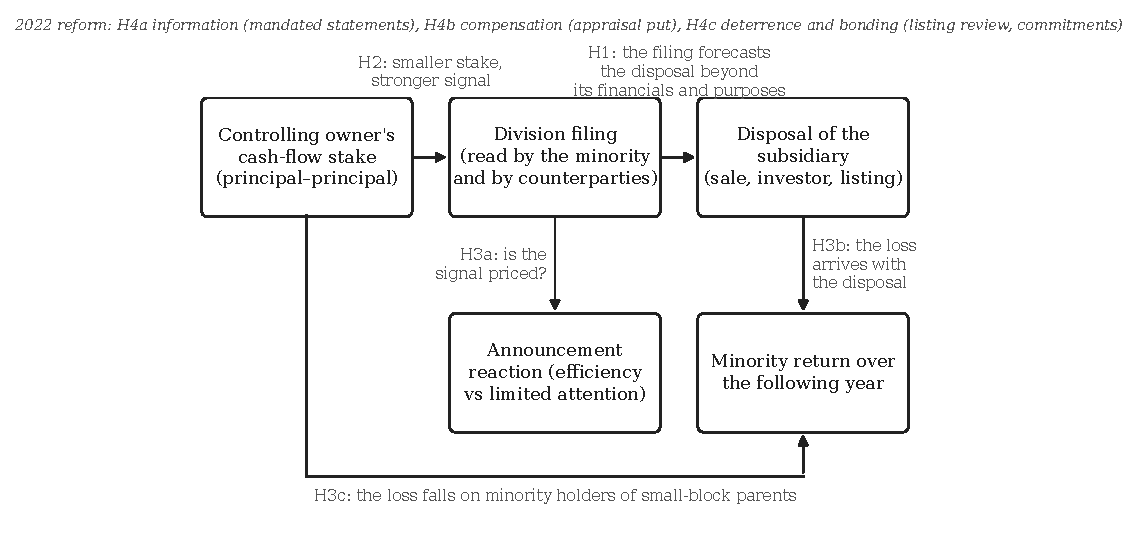
\includegraphics[width=\textwidth]{../figures/F1_framework_jifma.pdf}
\caption{The two steps of a \captive{} and the hypotheses}\label{fig:framework}
\tabnote{Boxes are the quantities the paper measures; arrows carry the hypotheses of Section~\ref{sec:setting}. H1 and H2 concern what the filing reveals and why; H3 concerns how the market and the minority's returns respond; H4a--c concern the three channels of the 2022 reform.}
\end{figure}

\begin{table}[htbp]
\centering
\caption{Hypotheses, rival predictions and tests}\label{tab:hyp}
{\scriptsize\singlespacing\setlength{\tabcolsep}{4pt}
\begin{tabular}{>{\raggedright\arraybackslash}p{1.5cm}>{\raggedright\arraybackslash}p{4.1cm}>{\raggedright\arraybackslash}p{3.7cm}>{\raggedright\arraybackslash}p{4.4cm}}
\toprule
Hypothesis & Prediction (theory) & Rival prediction & Test and exhibit \\
\midrule
H1 legibility & Filing text predicts disposal beyond financials and purpose categories; sharpest for early disposals (disclosure economics, verifiable statements) & No increment over financials (boilerplate) or over purpose categories (cheap talk) & Nested cross-validated models M0--M3 with bootstrap increments; Cox hazard with period strata; Table~\ref{tab:gate1}, Fig.~S1 \\
H2 stake & Smaller block $\rightarrow$ stronger signal, more disposals; block acts through the signal (principal--principal) & Block unrelated to signal and disposal (efficiency view) & Signal and disposal on the block with year, industry FE, firm clusters, foreign ownership, board; Table~\ref{tab:block} \\
H3 market & (a) lower announcement return and (b) no drift where the filing signals disposal (efficiency) & (a$'$) non-negative reaction, (b$'$) drift that arrives with the disposal, (c$'$) concentrated in small-block parents (limited attention) & Announcement CAR and one-year rank on the signal; benchmarks, FE, clusters, controls; realised early disposal; Table~\ref{tab:returns}, Fig.~\ref{fig:signal} \\
H4a information & Reaction rises relative to equity spin-offs; signal unchanged (mandated disclosure) & Signal falls, reaction falls (deterrence) & Captive $\times$ post DiD against equity spin-offs with placebo cut; Table~\ref{tab:reform}, Panel A \\
H4b compensation & Reaction rises with appraisal-price moneyness for post-reform captives only (put) & No slope anywhere (right not priced) & CAR on moneyness with pre-reform and equity-spin-off placebos; Table~\ref{tab:reform}, Panel C \\
H4c deterrence, bonding & Binding protection statements carry lower signal and fewer disposals (bonding) & Content unrelated to signal and disposal (cheap talk) & Protection-block categories and strength against the signal and labelled disposals; Table~\ref{tab:reform}, Panel B \\
\bottomrule
\end{tabular}}
\end{table}

\section{Data, measures and research design}\label{sec:data}

\subsection{Why these data, and the sample}\label{sec:sample}

The hypotheses need four things from the data, and the Korean record supplies each in a form that few other settings do. First, the filing that carries the controller's statements must be mandatory, public and comparable across firms and years: every Korean company that divides must file a division resolution with the Financial Supervisory Service's disclosure system, DART, and since 2017 the filing follows a structured form whose items---purpose, effects, the new company's assets and debt, listing application, put-option contracts---are the same for every filer, so the text can be read as a document and its stated financials used as the baseline that \eqref{eq:posterior} requires. Second, the outcome must be a discrete event the parent must later report: a Korean parent lists its equity investments, with the stake held, in every annual and half-year report, and the exchange records every listing, so whether the subsidiary was kept, sold or listed can be read for every division old enough to have reports. Third, the setting must offer an untreated comparison for the reform: equity spin-offs were filed under the same form in the same years and were exempt from all three measures. Fourth, an independent hand-coded sample should exist against which a model-read measure can be checked: \citeA{kang2025} coded the purposes and outcomes of \KLN{} listed-parent divisions of 2001--2021 by hand, and Section~\ref{sec:validity} compares our extractions with theirs. Prices come from the Korea Exchange for 2017--2026 and from Compustat Global for 2001--2016, the latter also supplying the universe of Korean common stocks from which the size and book-to-market benchmarks and the propensity-matched controls are drawn; ownership comes from the largest-shareholder table of the annual report; foreign holdings from the exchange's daily shareholding records.

The population is every \captive{} announced in a division resolution filed between 2001 and 2026, whether or not the parent was listed. For 2017 onward we take the structured division-resolution reports that DART returns (\NNewN{} divisions, \NMixed{} of which combined a captive with an equity spin-off). For 2001 to 2016, before the structured record exists, we retrieved every filing titled a division or division-and-merger resolution, clustered a filing and its corrections into one event, and had a language model extract the division's form with verbatim evidence; \NOldN{} events have a captive part. Divisions are dated by the receipt date of the original filing. The events pass through three measurements (Table~\ref{tab:sample}, Panel A): \NScored{} of the \NAllN{} events have a reading of the filing by both models, \NClean{} a clean outcome label (\NGateOne{} with the filing financials the baseline model needs), \NAllPriced{} listed parents have prices around the announcement and \NScoreOneY{} a full one-year window and a reading, a window being full when at least 90 percent of trading days $+2$ to $+250$ are priced. Panel B describes those \DescN{} parents, announced between \DescYearMin{} and \DescYearMax{} (\DescPeriodOld{} before 2017), \DescKosdaqPct{} percent of them KOSDAQ companies. The signal has a mean of \DescPLlmMean{} and a standard deviation of \DescPLlmSD{}; \DescDisposedPct{} percent of the labelled subsidiaries were disposed of and \DescEarlyRecPct{} percent of those with a recorded timing within a year; the mean three-day announcement return is \DescCarMmMPMean{} percent and the median one-year market-adjusted return \DescBharMadjPPMedian{} percent, against a mean of \DescBharMadjPPMean{}, the skew that motivates the rank specification below; the controlling block averages \DescBlockMean{} percent of common shares and foreign ownership \DescForeignMean{} percent with a median of \DescForeignMedian{}.

\begin{table}[htbp]
\centering
\caption{Sample construction and descriptive statistics}\label{tab:sample}
{\footnotesize\singlespacing\setlength{\tabcolsep}{3pt}
\emph{Panel A. From division filings to the analysis samples}\par\smallskip
% generated by code/make_tables_cgir.py (labels remapped by make_tables_jifma.py) on 2026-11-11 — source: carveout_disposal_tracking_{2001_2016,v4}.json; dart_division_decisions_2017_2026.json; event_study_meta_compustat.csv; ownership_pre_event_all.json; gate1_pooled_20261019.json by_source
\begin{tabular}{>{\raggedright\arraybackslash}p{9.2cm}rrr}
\toprule
 & 2001--2016 & 2017--2026 & Total \\
\midrule
Captive spin-off announcements with a tracked outcome file (listed and unlisted parents) & 464 & 294 & 758 \\
\quad disposed within the tracking window & 257 & 145 & 402 \\
\quad retained at 100\% & 89 & 90 & 179 \\
\quad merged back or liquidated (excluded) & 43 & 29 & 72 \\
\quad label unresolved or too recent (excluded) & 75 & 30 & 105 \\
Clean-label events with a disposal score (Table~\ref{tab:gate1}) & 345 & 234 & 579 \\
Listed parents with daily prices around the announcement & 380 & 260 & 640 \\
\quad with a full one-year post-announcement window & 366 & 249 & 615 \\
Parents with pre-announcement controlling-block ownership & 387 & 283 & 670 \\
\bottomrule
\end{tabular}
\par\medskip
\emph{Panel B. Listed parents with a signal and a full one-year return window}\par\smallskip
{\scriptsize% generated by code/make_tables_jifma.py on 2026-11-14 — source: data/processed/bhar_controls_events_20261025.csv (19), ownership_pre_event_all.json, event_governance_controls_20261110.csv (34); sample = signal and full one-year window
\begin{tabular}{>{\raggedright\arraybackslash}p{6.6cm}rrrrrr}
\toprule
Variable & $n$ & Mean & SD & P25 & Median & P75 \\
\midrule
Disposal signal $S$ (0--1) & 559 & 0.525 & 0.188 & 0.403 & 0.490 & 0.631 \\
Disposed (clean label, 0/1) & 469 & 0.70 & 0.46 & 0.00 & 1.00 & 1.00 \\
Disposed within a year (timing recorded, 0/1) & 405 & 0.48 & 0.50 & 0.00 & 0.00 & 1.00 \\
Announcement CAR $[-1,+1]$, \% & 546 & 0.6 & 8.4 & $-$3.3 & 0.2 & 3.6 \\
One-year market-adjusted BHAR, \% & 559 & $-$5.6 & 70.9 & $-$41.0 & $-$16.1 & 11.5 \\
Within-year rank of the BHAR (0--1) & 559 & 0.52 & 0.29 & 0.27 & 0.52 & 0.77 \\
Controlling block, \% of common shares & 524 & 35.0 & 19.1 & 21.5 & 34.8 & 46.6 \\
Foreign ownership at day $-1$, \% & 540 & 8.0 & 12.9 & 0.4 & 2.4 & 10.0 \\
Log market capitalisation (KRW) & 557 & 25.89 & 1.74 & 24.78 & 25.53 & 26.81 \\
Log book-to-market & 408 & $-$0.40 & 1.00 & $-$0.98 & $-$0.34 & 0.29 \\
Six-month pre-announcement market-adjusted return & 546 & 0.06 & 0.56 & $-$0.22 & $-$0.04 & 0.22 \\
KOSDAQ parent (0/1) & 559 & 0.47 & 0.50 & 0.00 & 0.00 & 1.00 \\
New company's share of combined assets & 317 & 0.13 & 0.12 & 0.04 & 0.10 & 0.19 \\
Surviving company's debt to assets & 324 & 0.41 & 0.21 & 0.25 & 0.41 & 0.57 \\
Listing application stated in the filing (0/1) & 559 & 0.002 & 0.042 & 0.000 & 0.000 & 0.000 \\
\bottomrule
\end{tabular}
}}
\tabnote{Panel A counts events at each stage of measurement, by filing era. Panel B describes the \DescN{} parents of the return regressions; variables are defined in Table~\ref{tab:defs} and Section~\ref{sec:returns}, returns in percent.}
\end{table}

The outcome is read from the parent's own later filings. We traced each new company by name (and by the name it took at incorporation) through the parent's annual and half-year reports for up to six fiscal years, to fiscal 2025 at the latest, and through the exchange's listing records. The subsidiary is disposed of when the parent sold a majority, listed it, or let its stake fall below 99.5 percent through a sale or a third-party investment, and retained when every report through the latest one, fiscal 2025 at the most recent, shows 100 percent; divisions after June 2025, which have no annual report to read, and divisions merged back, liquidated or too poorly documented to classify are excluded (\NAllOther{} and \NAllUnresolved{} events). A retained label is therefore right-censored---a 2024 division has one or two reports behind it, a 2010 division six---and the forecast's horizon of three to five years is met only for divisions up to about 2021; the hazard model of Section~\ref{sec:gate1} treats the censoring explicitly, and the period columns of Table~\ref{tab:gate1} and Table S6 give the older divisions alone. Under the 99.5 percent threshold a small third-party stake counts as a disposal; the labels that turn on it are flipped in Table S2. Of the \NClean{} clean-label events, \CleanDisposedShare{} percent were disposed of and \IPOShare{} percent listed; on listed parents of 2001--2021 our labels place \OurListedShare{} percent of subsidiaries in a listing and \OurRetainedShare{} percent retained at 100 percent, against \KLListed{} and \KLRetained{} percent in the independently built hand-coded sample of \citeA{kang2025}. A disposal is dated by the fiscal year of the report that first shows it, which separates disposals within a year of the division from later ones and gives the survival analysis its time scale. The 2017--2026 labels agree with a hand-maintained tracker on \LabelCrossAgree{} decided cases (\LabelCrossPct{} percent); \NSensitive{} depend on a definitional choice or a source conflict, and recoding all of them as retained changes no result (Table S2).

\subsection{The disposal signal}\label{sec:signal}

We estimate the reader's forecast $\pi_i$ of \eqref{eq:posterior} with two large language models from different vendors, Model~A, Anthropic's \texttt{claude-fable-5-1}, and Model~B, OpenAI's \texttt{gpt-6.1-sol}, both called through Amazon Bedrock under the identifiers \texttt{us.anthropic.claude-fable-5-1} and \texttt{us.openai.gpt-6.1-sol} between 15 and 25 October 2026, with extended reasoning and no sampling parameters altered. Each model reads the filing's full text and is told the filing's own date, so that its forecast is made as of that date; the reading stands for what a careful reader could have inferred then, a proxy whose validity Section~\ref{sec:validity} tests. Text measures of disclosure content have moved from word lists \cite{loughran2011} to supervised learning \cite{frankel2022} and to language models \cite{siano2025}; ours asks for a forecast of a specific event that we later observe, not a tone score. Each model is instructed to forecast, from the document alone and without using anything it may know about the company's later history, the probability that the parent will not retain 100 percent of the new company within roughly three to five fiscal years, and to return it as an integer from 0 to 100 together with the most likely route, reasons, verbatim supporting sentences, and the facts stated in the filing (purposes from a fixed list of seven categories; whether a listing, an outside investor, a sale or buyer, protection measures and the appraisal right are mentioned; the new company's business and capital). The disposal signal of filing $i$ is the two models' probabilities averaged and rescaled to the unit interval,
\begin{equation}\label{eq:signal}
S_i = \frac{1}{2}\sum_{m\in\{A,B\}}\frac{1}{R_m}\sum_{r=1}^{R_m}\frac{p_{i,m,r}}{100},
\end{equation}
where $R_m$ is the number of runs (two for 2017--2026, one for 2001--2016). It is judged against the realised label $D_i$ by the area under the ROC curve, $\mathrm{AUC} = \Pr(S_i > S_j \mid D_i = 1, D_j = 0)$, and enters the return tests as a level or as its within-year rank. The prompts, parsing code and every judgment are in the replication archive, so the tables regenerate without a model call.

\subsection{Measurement validity and bias of the signal}\label{sec:validity}

Because $S$ is produced by a model rather than by a hand-coded rule we treat it as a measured variable with error and ask of it what one would ask of any new measure: whether it is stable, whether it could have been contaminated, for whom it works less well, whether its errors line up with firm characteristics, and whether its ingredients agree with hand coding (Table S1; predictive validity is Section~\ref{sec:gate1}).

Re-running each model reproduces $S$ with correlations of \RepeatCorrA{} and \RepeatCorrB{}. Across vendors the probabilities correlate at \TwoModelCorr{} over the \TwoModelN{} filings with a first-run judgment from both models (three of the \NScored{} scored filings have Model~A's reading from a repeat run only), and the models differ in level (means \TwoModelMeanA{} and \TwoModelMeanB{}), which is why we average and rank within year.

A model that recognises the firm could ``predict'' an outcome it has read about \cite{glasserman2024}, so every filing was re-read with the parent's and new company's names, group names, tickers and dates removed. The anonymised reading has an AUC of \ValAUCAn{} against \ValAUCId{} for the identified first-run reading of the same filings (the two-run average of Section~\ref{sec:signal} reaches \AUCPooledLLM{}); the paired-bootstrap difference is \ValDAUC{} with interval [\ValDAUCLo, \ValDAUCHi], and at most \ValDAUCMaxSub{} in any subgroup. Model~A reported drawing on outside knowledge for \ValSubsetN{} of the \ValOutsideN{} labelled filings for which it returned the field (\ValOutsideA{} percent; Model~B reported it for \ValOutsideB{} percent), and inside that subset the identified and anonymised readings are equally accurate (\ValSubsetAUCId{} against \ValSubsetAUCAn{}). The anonymised signal reproduces the return results (Supporting Information). Anonymisation removes the recall of a firm; it does not remove what a model trained to 2026 knows about how division filings tend to end. A careful human reader in 2010 brought the same kind of knowledge, in smaller measure, and the only test that separates the two is a blind human reading of a sample of filings, which we have prepared but not run (Section~\ref{sec:conclusion}).

Discrimination is similar across exchanges (\ValAUCKosdaqKosdaq{} and \ValAUCKosdaqKospiOther{}) and weaker for filings before 2009 (\ValAUCPeriodEarly{} against \ValAUCPeriodLate{} after 2016), for unlisted parents (\ValAUCListedUnlisted{} against \ValAUCListedListed{}; interaction $p$ = \ValLRDiscListed{}) and for the smallest third of parents by filing assets (\ValAUCSizeSmall{} against \ValAUCSizeMid{}--\ValAUCSizeLarge{}; $p$ = \ValLRDiscSize{}). The signal is conservative everywhere (mean \ValMeanS{} against a realised disposal rate of \ValMeanY{}), most so for small parents. The part of $S$ that the models' own extracted facts, text length and period do not explain (stage-one $R^2$ \ValStageOneRTwo{}) has no standardised association with size, exchange, listing status, relative size or foreign ownership above \ValMaxBeta{}; the one pattern is that the error $S - D$ rises with parent size (\ValErrSizeBeta{}, $p$ = \ValErrSizeP{}). The signal is not inflated for large, listed or foreign-held firms; if anything it under-reads small parents, whose disposal rate is highest, and the return tests carry size, exchange, listing and industry controls.

The two models agree on the facts that enter the signal's decomposition (sale purpose $\kappa$ = \KappaSale{}, fund-raising \KappaFund{}, holding-company restructuring \KappaHolding{}, a named sale or buyer \KappaBuyer{}) and disagree only where a field's boundary is ambiguous (whether the form's ``re-listing application: no'' counts as a mention of listing, $\kappa$ = \KappaListing{}), fields we do not use. Against the hand coding of \citeA{kang2025} on the same population, our listed-parent filings of 2001--2021 show a stated sale purpose in \OurSaleStrict{} percent (\OurSaleBroad{} counting fund-raising) against their \KLSale{}; their near-universal specialisation code (\KLSpecial{} percent) and rare efficiency code (\KLEff{}) are not comparable with a multi-label extraction that records both for almost every filing.

\subsection{Returns, ownership and controls}\label{sec:returns}

For listed parents day 0 is the first trading day on or after the receipt date of the original filing. The announcement return is the market-model cumulative abnormal return over days $-1$ to $+1$, estimated over days $-250$ to $-31$ against the parent's market index; the one-year return is the parent's buy-and-hold return minus the benchmark's over days $+2$ to $+250$,
\begin{equation}\label{eq:bhar}
\mathrm{BHAR}_i = \prod_{\tau=2}^{250}(1+R_{i\tau}) - \prod_{\tau=2}^{250}(1+R_{B\tau}),
\end{equation}
with $B$ the market index in the main specification and the parent's size and book-to-market portfolio or a matched firm in the benchmark tests. Windows with fewer than 90 percent of trading days are dropped. Daily adjusted prices for 2017--2026 come from the Korea Exchange and for 2001--2016 from Compustat Global, whose returns match the exchange's on the overlap (median daily correlation \KRXCompustatCorr{}); \GlitchExcluded{} parents whose Compustat window contains a return beyond the exchange's price limit without a delisting are excluded. Because long-run returns are skewed \cite{barber1997, lyon1999, fama1998, mitchell2000}---Panel B of Table~\ref{tab:sample} puts the mean one-year return at \DescBharMadjPPMean{} percent and the median at \DescBharMadjPPMedian{}---the headline dependent variable is the parent's percentile rank of the one-year return within its announcement year, with means and medians beside it.

The controlling block at the fiscal year-end before the announcement year is $\mathrm{Block}_i = 100\,(H_i - T_i)/N_i$, where $H_i$ is the common shares held by the largest shareholder and the related parties listed with it, $T_i$ the treasury shares within that group and $N_i$ the shares outstanding; for announcements before 2016 two models read the table from the annual report and agree within one percentage point in \OwnWithinOne{} of \OwnPairs{} cases. The median block is \BlockMedian{} percent. The controls are the parent's log market capitalisation at the last month-end before the announcement and its log book-to-market (Compustat Global), its market-adjusted return over the six months before the announcement, its market, the new company's assets relative to the surviving company's, the surviving company's debt-to-assets ratio and whether the filing states a listing application; we add foreign ownership at day $-1$ from the exchange's shareholding records (\ForeignCoverage{} events; median \ForeignMedian{} percent) and, for fiscal years from 2014, the share of outside directors on the parent's registered board (\BoardN{} events; median \BoardMedian{}). Missing controls are set to the sample median with an indicator, and continuous controls are winsorised at the first and ninety-ninth percentiles. The regressions take the form
\begin{equation}\label{eq:main}
y_i = \alpha_{t(i)} + \alpha_{j(i)} + \beta\, S_i + \boldsymbol{\gamma}'\mathbf{x}_i + \varepsilon_i,
\end{equation}
with announcement-year effects $\alpha_t$, GICS-sector effects $\alpha_j$ where stated, and standard errors clustered by parent (two-way by parent and year where stated) beside the HC1 errors of the baseline; $\beta$ estimates $b_A$ of \eqref{eq:market} when $y_i$ is the announcement return and $b_Y$ when it is the one-year return or its rank. Table~\ref{tab:defs} collects the ten measures in one-sentence form; Table S9 in the Supporting Information gives the same ten rows, in the same order, with the full operational rules, sources and exclusions.

\begin{table}[htbp]
\centering
\caption{Definitions of the measures used in this paper (short form)}\label{tab:defs}
{\scriptsize\singlespacing\setlength{\tabcolsep}{3pt}% generated by code/make_tables_cgir.py (labels remapped by make_tables_jifma.py) on 2026-11-14 — source: DEFS list in code/make_tables_cgir.py (one row list; full form S_defs_full)
\begin{tabular}{>{\raggedright\arraybackslash}p{0.6cm}>{\raggedright\arraybackslash}p{3.1cm}>{\raggedright\arraybackslash}p{7.6cm}>{\raggedright\arraybackslash}p{3.4cm}}
\toprule
No. & Term & Definition & Applied in \\
\midrule
D1 & Captive spin-off (\emph{mulchŏk bunhal}) & A division in which the parent receives all shares of the new company; the parent's shareholders receive none. & Table~\ref{tab:sample}; all tests \\ \addlinespace[1pt]
D2 & Disposal & The parent ceases to hold about 100\% of the new company within the tracking window: sale of a majority, listing, or a stake sale or third-party investment taking the stake below 99.5\%. & Tables~\ref{tab:sample}, \ref{tab:gate1}, \ref{tab:returns} \\ \addlinespace[1pt]
D3 & Early disposal & First ownership change recorded in the fiscal year of the division or the next. & Tables~\ref{tab:returns}, \ref{tab:block} \\ \addlinespace[1pt]
D4 & Disposal signal & The probability of disposal that two language models assign to the announcement filing, averaged. & Tables~\ref{tab:gate1}, \ref{tab:returns} \\ \addlinespace[1pt]
D5 & Anonymised condition & The same filing with parent and new-company names, group prefixes and dates masked, and the filing date withheld. & Table~\ref{tab:gate1} \\ \addlinespace[1pt]
D6 & Controlling block & Common shares held by the largest shareholder and related parties, as a percentage of common shares, at the fiscal year-end before the announcement year; treasury shares excluded. & Table~\ref{tab:block} \\ \addlinespace[1pt]
D7 & Announcement CAR & Market-model cumulative abnormal return over trading days $-1$ to $+1$ around the filing date. & Tables~\ref{tab:returns}, \ref{tab:reform} \\ \addlinespace[1pt]
D8 & One-year BHAR & Buy-and-hold return of the parent minus that of its market index over trading days $+2$ to $+250$. & Tables~\ref{tab:returns}--\ref{tab:block} \\ \addlinespace[1pt]
D9 & Within-year rank & Percentile rank of the one-year BHAR among the year's events (0--1). & Tables~\ref{tab:returns}, \ref{tab:block} \\ \addlinespace[1pt]
D10 & Post-reform period & Filings received on or after 1 October 2022. & Table~\ref{tab:reform} \\ \addlinespace[1pt]
\bottomrule\end{tabular}
}
\tabnote{Short form; Table S9 gives the same ten rows, in the same order, with data fields, timing rules and exclusions. Both tables are generated from one row list in the replication archive.}
\end{table}

\subsection{Research design}\label{sec:design}

Several alternative explanations stand between the associations and the readings we give them; Table~\ref{tab:design} pairs each with the device that addresses it, and three of the devices are described here because the tables do not show them.

\emph{Benchmarks and selection.} From Compustat Global we build the universe of Korean common stocks and, for every event, a $5\times5$ size and book-to-market portfolio, a $3\times3$ portfolio, a matched firm nearest in size and book-to-market, and a propensity-matched control drawn from a firm-year logit of the division decision on lagged size, Tobin's $q$, leverage, investment, cash flow, cash, sales growth and market (\SelFirmYears{} firm-years, \SelEvents{} events; every event lies inside the controls' support; Table S3). The $5\times5$ assignment falls back to the size quintile when the book-to-market cell is empty; a strict variant drops those events.

\emph{Survival.} Because labels are censored at fiscal 2025 and disposals arrive at different speeds, we estimate a Cox model of the time from division to first disposal, measured in fiscal years and stratified by filing period $s \in \{2001\text{--}08, 2009\text{--}16, 2017\text{+}\}$,
\begin{equation}\label{eq:cox}
h_i(t) = h_{0,s(i)}(t)\, \exp\!\big(\beta_S S_i + \beta_B\, \mathrm{Block}_i + \boldsymbol{\gamma}'\mathbf{x}_i\big),
\end{equation}
with ties handled by Efron's method and parent-clustered errors; a subsidiary retained through its latest report is censored there. The hazard ratio per standard deviation of $S$ is $\exp(\beta_S\,\sigma_S)$. Two controls accompany the estimate: a permuted signal, whose ratio should cover one, and a synthetic sample with a known ratio that the estimator should recover.

\emph{Reform channels.} The information channel is a difference-in-differences on division announcements by listed parents,
\begin{equation}\label{eq:did}
\mathrm{CAR}_i = \alpha_{t(i)} + \delta_1\, \mathrm{Captive}_i + \delta_2\, \mathrm{Post}_i + \delta_3\, \mathrm{Captive}_i \times \mathrm{Post}_i + \boldsymbol{\gamma}'\mathbf{x}_i + \varepsilon_i ,
\end{equation}
with equity spin-offs as the control, $\mathrm{Post}_i$ equal to one for filings received on or after 1 October 2022, year effects, log market capitalisation and a KOSDAQ indicator, HC1 and parent-clustered errors, a placebo cut at October 2019 inside the pre-period, and a 21-day variant; $\delta_2$ enters on its own because calendar-year effects do not absorb a cutoff inside 2022. The compensation channel regresses the CAR of post-reform \captive{}s on the moneyness $m_i$ of \eqref{eq:moneyness} read from the appraisal price stated in the filing (\AppraisalPrices{} filings; the stated price matches the decree formula within \AppraisalProxyDiff{} percent at the median where the board date lies within a month of the filing), with the formula ratio as a placebo where no right existed, and compares the ex-post payoff of dissenting, $K_i / P_{i,-1} - 1$, with the return to holding the parent for a year. The deterrence and bonding channel classifies the mandatory protection block of every post-reform filing by its content and by the strength of its strongest commitment, and relates both to $S$ and to labelled disposals.

Every analysis was run from a memo that stated the expected range of each estimate before the first run; an estimate outside its range was first checked for code and data errors, and the memos, the log of what was changed and every estimate that moved are in the replication archive. Those that stayed outside their range after checking are reported as they came: the KOSDAQ coefficient of the selection model has the opposite sign to \citeA{kang2025}'s and is insignificant (\SelKosdaq{}, $p$ = \SelKosdaqP{}; Table S3); the signal's AUC spreads more across subgroups than the 0.15 we had allowed (\ValAUCSizeSmall{} for the smallest parents; Table S1); and filings with a charter clause carry a mean signal of \ProtMeanSCharter{}, not the value below 0.40 we expected (Table~\ref{tab:reform}).

\begin{table}[htbp]
\centering
\caption{Research design: alternative explanations and devices}\label{tab:design}
{\scriptsize\singlespacing\setlength{\tabcolsep}{4pt}
\begin{tabular}{>{\raggedright\arraybackslash}p{3.0cm}>{\raggedright\arraybackslash}p{5.4cm}>{\raggedright\arraybackslash}p{6.3cm}}
\toprule
Concern & Alternative explanation & Device (exhibit) \\
\midrule
Model recall & The model remembers the firm's later history & Name- and date-anonymised re-reading; self-reported outside knowledge; subgroup $\Delta$AUC (Sec.~\ref{sec:validity}; Table S1) \\
Measurement bias & The signal is inflated for some kinds of firms & Subgroup AUC and calibration; residual-bias regressions; two-model agreement; external hand-coded benchmark (Table S1) \\
Contribution over hand coding & The signal restates purpose categories or keywords & Nested models M0--M3 with paired-bootstrap increments; keyword and facts-only ladders (Table~\ref{tab:gate1}) \\
Label censoring & Young divisions look ``retained'' & Cox model with period strata, eq.~\eqref{eq:cox}; Kaplan--Meier by tercile (Table~\ref{tab:gate1}, Fig.~S1) \\
Omitted firm condition & A troubled parent writes a disposal-like filing and underperforms & Size, value, momentum, leverage, foreign ownership, board; realised early disposal beside the signal (Tables~\ref{tab:returns}, \ref{tab:block}) \\
Industry; repeat filers & Industry cycles; the same parent files repeatedly & Year + GICS-sector fixed effects; parent- and two-way-clustered errors (Tables~\ref{tab:returns}, \ref{tab:block}, S4) \\
Benchmark & Market-adjusted returns load on size and value & $5\times5$ and $3\times3$ size/B-M portfolios, matched firm, propensity-matched control (Table~\ref{tab:returns}, Panel C) \\
Selection into division & Dividing firms differ from the universe & Firm-year selection logit on the Compustat Global universe; propensity support; matched controls (Table S3) \\
Reform confounded with time & 2023--2026 markets differ & Equity spin-offs as untreated control, eq.~\eqref{eq:did}; placebo cut; 2001--2026, winsorised, median and 21-day variants (Table~\ref{tab:reform}) \\
Reform is a package & The three measures arrived within one quarter & The DiD is read as the package's effect; each channel is tested by the distinct trace it would leave (Table~\ref{tab:reform}, Panels A--C) \\
Right not priced; statements cheap & Appraisal right and protection statements are formalities & Moneyness slope with two placebos; protection-block content vs signal and disposals (Table~\ref{tab:reform}) \\
Label error & Model-read labels are wrong & Tracker cross-check; definition-sensitive labels flipped and dropped (Table S2) \\
\bottomrule
\end{tabular}}
\end{table}

\section{Results}\label{sec:results}

\subsection{The filing is legible (H1)}\label{sec:gate1}

Table~\ref{tab:gate1}, Panel A, is the ladder of nested models. On the \NGateOne{} clean-label divisions a cross-validated logistic model on the filing's financial covariates orders disposed from retained subsidiaries with an AUC of \NestedMZero{}, no better than chance in 2001--2016 (\NestedMZeroOld{}). Adding the seven stated-purpose categories that a hand coder would record, the categories \citeA{kang2025} used, raises it to \NestedMOne{} (increment \NestedIncMOneMZero{}); adding the five mention flags---buyer, outside investor, listing, protection measures, appraisal right---adds little more (\NestedMTwo{}). Adding the disposal signal raises the model to \NestedMThree{}, an increment of \NestedIncMThreeMTwo{} with a paired-bootstrap interval of [\NestedIncMThreeMTwoLo, \NestedIncMThreeMTwoHi] and a likelihood-ratio $p$ \NestedLRpMThree{}; the signal alone reaches \NestedS{}, and keyword flags read from the raw text without any model add \NestedIncKOneMZero{} to the financial baseline. The holistic reading is therefore not a finer version of the purpose code: the facts a coder extracts explain \DecompRTwo{} of the variance of $S$---the sale-purpose category alone moves it by \DecompSaleCoef{} and fund-raising by \DecompFundCoef{}---and the residual, what the models read beyond those facts, orders the outcomes with an AUC of \DecompAUCResid{} on its own. Permuting the labels returns mean cross-validated AUCs between \PermAUCMin{} and \PermAUCMax{} for every model. The content that carries the information is the counterparty-addressed statement the disclosure strand predicts: Doosan's 2021 filing stated that the parent would sell its entire stake in the new company to an affiliate (signal \ExDoosanScore{}; \ExDoosanOutcome{}); CJ ENM's 2020 filing listed ``attracting outside investment \ldots{} and the sale of shares where necessary'' among its purposes (\ExTvingScore{}; \ExTvingOutcome{}); DB HiTek's 2023 filing wrote a shareholder vote before any listing into both companies' charters (\ExDBScore{}; \ExDBOutcome{}).

\begin{table}[htbp]
\centering
\caption{The filing predicts the disposal: nested models and the hazard of disposal}\label{tab:gate1}
{\footnotesize\singlespacing\setlength{\tabcolsep}{3pt}
\emph{Panel A. Cross-validated AUC of nested disposal models}\par\smallskip
% generated by code/make_tables_jifma.py on 2026-11-14 — source: results/nested_models_20261110.json -> ladder_pooled, ladder_by_period, increments
\begin{tabular}{l>{\raggedright\arraybackslash}p{6.0cm}cccrr}
\toprule
Model & Inputs & CV AUC & Brier & $\Delta$AUC [95\% CI] & 2001--2016 & 2017+ \\
\midrule
M0 & Financial covariates of the filing & 0.587 & 0.209 & -- & 0.445 & 0.581 \\
M1 & M0 + stated-purpose categories (Kang--Lee type) & 0.667 & 0.200 & +0.080 [0.044, 0.115] & 0.566 & 0.668 \\
M2 & M1 + mention flags (buyer, investor, listing, protection, appraisal) & 0.680 & 0.198 & +0.013 [$-$0.014, 0.039] & 0.599 & 0.733 \\
M3 & M2 + disposal signal $S$ & 0.770 & 0.170 & +0.091 [0.052, 0.128] & 0.706 & 0.830 \\
F & Extracted facts only (purpose + mentions) & 0.611 & 0.205 & -- & 0.593 & 0.689 \\
K1 & M0 + keyword flags read from the raw text, no model & 0.590 & 0.210 & +0.003 [$-$0.026, 0.028] & 0.521 & 0.600 \\
S & Signal alone & 0.758 & 0.172 & -- & 0.700 & 0.809 \\
\bottomrule
\end{tabular}
\par\medskip
\emph{Panel B. Cox model of the time from division to first disposal}\par\smallskip
% generated by code/make_tables_jifma.py on 2026-11-14 — source: results/cox_time_to_disposal_20261110.json -> models.A.cox_strata_period, kaplan_meier_sample_A, expectation_check.HR_S_per_sd
\begin{tabular}{lcccc}
\toprule
 & HR & 95\% CI & $p$ & \\
\midrule
Disposal signal $S$, per standard deviation & 1.96 & [1.74, 2.19] & $<$0.001 & \\
Controlling block, per 10 pp & 0.964 & [0.908, 1.024] & 0.232 & \\
Relative size of the new company & 4.54 & [1.23, 16.75] & 0.023 & \\
Parent leverage after the division & 2.70 & [1.28, 5.70] & 0.009 & \\
log new-company assets & 0.852 & [0.772, 0.941] & 0.002 & \\
KOSDAQ parent & 1.001 & [0.775, 1.292] & 0.993 & \\
\midrule
Kaplan--Meier share disposed by signal tercile & by year 1 & by year 3 & by year 5 & $n$ \\
\midrule
Low $S$ (0.13--0.44) & 24\% & 33\% & 39\% & 163 \\
Middle (0.44--0.57) & 54\% & 74\% & 82\% & 160 \\
High $S$ (0.57--0.99) & 74\% & 83\% & 85\% & 161 \\
\bottomrule
\end{tabular}
}
\tabnote{Panel A: logistic models of the clean-label disposal indicator on the \NGateOne{} divisions, estimated with repeated stratified five-fold cross-validation (50 repeats); M0 uses the characteristics stated in the filing (new company's assets, debt to assets and sales to assets; relative size; surviving company's debt to assets; listing application; put-option contract; market). Purpose categories and mention flags are the majority vote of the models' structured extractions; keyword flags are regular-expression matches on the raw text. $\Delta$AUC is the paired-bootstrap increment over the preceding row (K1 over M0). Panel B: Cox proportional-hazards model stratified by period (2001--08, 2009--16, 2017+) on \CoxN{} divisions with a recorded disposal year (\CoxEvents{} disposals; concordance \CoxConcordance{}); time is the fiscal year of the first ownership change, censored at the latest report. The hazard ratio of $S$ per standard deviation is the per-unit ratio raised to the sample standard deviation of $S$. Kaplan--Meier shares are the cumulative proportion disposed of by the end of the stated fiscal year after the division.}
\end{table}

Panel B treats the censoring of young labels directly. In a Cox model of the time from division to first disposal, stratified by period and conditional on the filing controls and the block, the hazard of disposal rises by a factor of \CoxHRSD{} per standard deviation of the signal (95 percent interval \CoxHRSDLo--\CoxHRSDHi); a permuted signal returns a ratio of \CoxPermHR{} with an interval covering one, and a synthetic sample with a known ratio recovers it. The Kaplan--Meier shares in Panel B (drawn in Figure S1) put the ratio in shares: within one fiscal year of the division \KMLowOneY{} percent of the subsidiaries in the lowest tercile of the signal had changed hands, against \KMMidOneY{} in the middle and \KMHighOneY{} in the top tercile; the baseline hazard is front-loaded (\KMAllOneY{} percent of all subsidiaries within a year, \KMAllFiveY{} within five), so the first year after a division is when the controller's intention is executed, and the filing is sharpest about exactly those disposals (AUC \AUCEarlyPooled{} for disposals within a year against the retained, \AUCLateVsNever{} for disposals two or more years later). The controlling block, conditional on the signal, has a hazard ratio of \CoxHRBlock{} per ten percentage points (\CoxHRBlockLo--\CoxHRBlockHi): what the block tells us about the disposal is already in the filing, the chain H2 predicts.


\subsection{The market's reaction and the year after (H3)}\label{sec:market}

The announcement reaction does not fall with the disposal signal; it rises. With year fixed effects the slope of the three-day abnormal return on the signal is \AnnCarSlope{} ($p$ = \AnnCarSlopeP{}), so a filing that reads as a certain disposal is received \AnnCarSlopePP{} percentage points more favourably than one that reads as a certain retention (Table~\ref{tab:returns}, Panel B); the slope is \AnnSSector{} with GICS-sector effects and parent-clustered errors ($p$ = \AnnSSectorP{}) and \AnnSPlusPurposeMentions{} once the purpose and mention dummies are added ($p$ = \AnnSPlusPurposeMentionsP{}), so the favourable reception attaches to the stated growth story rather than to the residual reading. The return over the following year falls with the signal. The Spearman correlation between the signal and the one-year market-adjusted return is \SpearmanScoreBhar{} across \NScoreOneY{} parents ($p$ = \SpearmanScoreBharP{}); the median return in the top quintile of the signal is \QFiveMedian{} percent against \QOneMedian{} in the bottom quintile (Figure~\ref{fig:signal}). Panel A of Table~\ref{tab:returns} carries the within-year rank of the return across specifications. The coefficient on the signal is \RankSpecThreeCoef{} with year effects, HC1 errors and the full controls, which places a filing at the disposal end of the signal \RankSpecThreePctl{} percentiles lower in its year's ranking than one at the retention end; it is \RankSSector{} with year and GICS-sector effects and parent-clustered errors ($p$ = \RankSSectorPFirm{}; \RankSSectorPTwoway{} with two-way clustering), \RankSPlusPurposeMentions{} with the purpose and mention dummies added ($p$ = \RankSPlusPurposeMentionsP{})---the drift attaches to the reading, not to the categories---and \RankSForeign{} with foreign ownership added ($p$ = \RankSForeignP{}; foreign ownership itself is unrelated to the rank). On the 2015+ subsample with the outside-director ratio the coefficient is \RankSBoard{} ($n$ = \RankSBoardN{}, $p$ = \RankSBoardP{}), imprecise rather than smaller.

\begin{table}[htbp]
\centering
\caption{Returns on the disposal signal: specifications and benchmarks}\label{tab:returns}
{\footnotesize\singlespacing\setlength{\tabcolsep}{3pt}
% generated by code/make_tables_jifma.py on 2026-11-11 — source: results/industry_fe_firm_clusters_20261110.json -> table6_returns_on_signal; nested_models_20261110.json -> return_ladder; governance_controls_20261110.json -> regressions
\begin{tabular}{l>{\raggedright\arraybackslash}p{7.2cm}ccr}
\toprule
 & Specification & Coefficient on $S$ (s.e.) & $p$ & $n$ \\
\midrule
\multicolumn{5}{l}{\emph{Panel A. Within-year rank of the one-year market-adjusted BHAR}} \\
(1) & Year FE, HC1 & $-$0.195 (0.068) & 0.004 & 559 \\
(2) & Year + GICS sector FE, firm cluster & $-$0.194 (0.067) & 0.004 & 559 \\
(3) & Year + GICS sector FE, two-way cluster & $-$0.194 (0.046) & $<$0.001 & 559 \\
(4) & (1) + Kang--Lee-type purpose and mention dummies & $-$0.296 (0.085) & $<$0.001 & 559 \\
(5) & (1) + foreign ownership & $-$0.211 (0.069) & 0.002 & 540 \\
(6) & (1) + foreign ownership + outside-director ratio (FY2015+) & $-$0.187 (0.121) & 0.119 & 194 \\
\midrule
\multicolumn{5}{l}{\emph{Panel B. Three-day announcement CAR}} \\
(7) & Year FE, HC1 & 0.039 (0.019) & 0.041 & 560 \\
(8) & Year + GICS sector FE, firm cluster & 0.045 (0.019) & 0.020 & 560 \\
(9) & (7) + Kang--Lee-type purpose and mention dummies & 0.037 (0.024) & 0.121 & 560 \\
(10) & (7) + foreign ownership & 0.041 (0.020) & 0.044 & 546 \\
\bottomrule
\end{tabular}
\par\medskip
\emph{Panel C. One-year returns against alternative benchmarks}\par\smallskip
{\scriptsize% generated by code/make_tables_jifma.py on 2026-11-11 — source: results/matched_benchmark_selection_20261110.json -> by_benchmark
\begin{tabular}{>{\raggedright\arraybackslash}p{4.6cm}rcccc}
\toprule
Benchmark & $n$ & Mean BHAR, \% [95\% CI] & Spearman($S$) ($p$) & Rank coef.\ on $S$ ($p$) & Early $-$ never, pp ($p$) \\
\midrule
Market-adjusted (paper) & 559 & $-$5.6 [$-$11.1, +0.4] & $-$0.137 (0.001) & $-$0.195 (0.004) & $-$13.6 (0.002) \\
5$\times$5 size/B-M portfolio (size fallback) & 540 & $-$8.2 [$-$13.5, $-$2.3] & $-$0.090 (0.036) & $-$0.147 (0.031) & $-$10.0 (0.069) \\
5$\times$5 strict & 513 & $-$7.7 [$-$13.4, $-$1.5] & $-$0.073 (0.101) & $-$0.117 (0.095) & $-$9.6 (0.118) \\
3$\times$3 size/B-M portfolio & 513 & $-$8.1 [$-$13.8, $-$1.8] & $-$0.085 (0.056) & $-$0.164 (0.019) & $-$8.8 (0.075) \\
Matched firm (size, B/M) & 504 & $-$8.6 [$-$17.6, +0.3] & $-$0.026 (0.555) & $-$0.017 (0.820) & $-$9.4 (0.316) \\
Propensity-matched control firm & 522 & $-$3.6 [$-$11.2, +3.7] & $-$0.088 (0.045) & $-$0.124 (0.071) & $-$15.1 (0.027) \\
\bottomrule
\end{tabular}
}}
\tabnote{Panels A and B: OLS coefficient on the disposal signal (0--1) with the standard error in parentheses. All specifications include announcement-year fixed effects and the controls of Section~\ref{sec:returns} (log market capitalisation, log book-to-market, six-month pre-announcement market-adjusted return, KOSDAQ, relative size of the new company, surviving company's debt to assets, stated listing application; missing values at the median with indicators). (2), (3) and (8) add GICS-sector fixed effects of the parent from Compustat Global; the $p$-value in (2) and (8) uses parent-clustered errors, in (3) two-way parent-and-year clustering; (4) and (9) add the seven purpose-category and five mention dummies of Table~\ref{tab:gate1}; (5), (6) and (10) add foreign ownership at day $-1$ and, in (6), the outside-director ratio. Panel C: the one-year BHAR of the same parents against each benchmark; the rank coefficient is from specification (1) with the within-year rank of the benchmark-adjusted return as dependent variable ($p$ parent-clustered); early $-$ never is the difference in mean BHAR between subsidiaries disposed of within a fiscal year and those retained (Mann--Whitney $p$). The $5\times5$ portfolio falls back to the size quintile when the book-to-market cell is empty; the strict row drops those events.}
\end{table}

Panel C asks whether the drift is the benchmark. Against the parent's $5\times5$ size and book-to-market portfolio the mean one-year abnormal return is \BenchPfSizebmWithSizeFallbackMean{} percent, the rank coefficient on the signal \BenchPfSizebmWithSizeFallbackRank{} ($p$ = \BenchPfSizebmWithSizeFallbackRankP{}) and the Spearman correlation \BenchPfSizebmWithSizeFallbackRho{}; against the $3\times3$ portfolio the coefficient is \BenchPfRank{} ($p$ = \BenchPfRankP{}), and against a propensity-matched control firm \BenchPsmControlFirmRank{} ($p$ = \BenchPsmControlFirmRankP{}). Against a single matched firm the association disappears (\BenchMatchedFirmSizebmRank{}, $p$ = \BenchMatchedFirmSizebmRankP{}); a one-firm benchmark is noisy, but the result depends on the benchmark being a portfolio, and we say so. The loss is realised where the signal said it would be: parents whose subsidiary changed hands within a fiscal year trail those that retained it by \EarlyNeverDiff{} percentage points against the market (Mann--Whitney $p$ = \EarlyNeverMWP{}) and by comparable margins against the portfolios, the coefficient of realised early disposal on the within-year rank is \EarlySector{} with sector effects and parent clusters ($p$ = \EarlySectorP{}), and when early disposal and the signal enter the rank regression together the signal's coefficient falls to \JointScoreCoef{} ($p$ = \JointScoreP{}): the signal's information about the return is the information it carries about the early disposal. The pattern is the limited-attention rival of H3---(a$'$), (b$'$)---and not the efficient reading.

\begin{figure}[htbp]
\centering
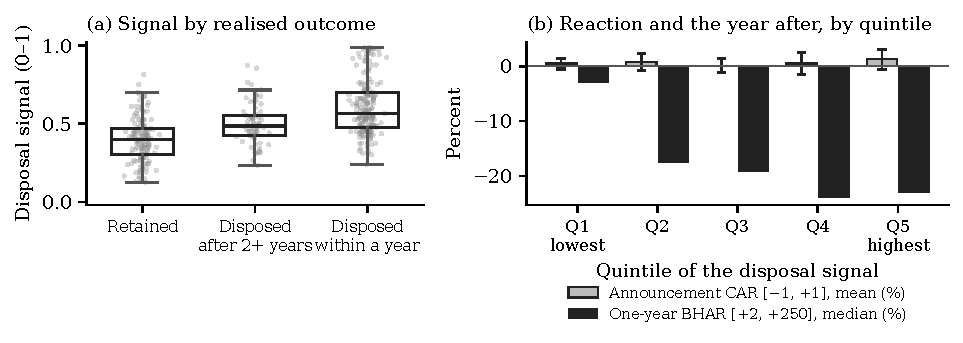
\includegraphics[width=0.86\textwidth]{../figures/F2_signal_outcomes.pdf}
\caption{The disposal signal, realised outcomes and returns}\label{fig:signal}
\tabnote{Panel (a): the two-model disposal signal of the listed parents with a full one-year window, by realised outcome and timing (boxes: interquartile range and median; points: events). Panel (b): mean three-day announcement CAR with bootstrap 95 percent intervals and median one-year market-adjusted BHAR by quintile of the signal.}
\end{figure}

\subsection{The controlling owner's stake (H2 and H3c$'$)}\label{sec:block}

Parents with small controlling blocks wrote the filings that read most as disposals, disposed most often and earned least. In the lowest tercile of the block (up to \LowBlockMax{} percent of common shares) \LowBlockDisp{} percent of subsidiaries were disposed of and \LowBlockEarly{} percent within a year, against \HighBlockDisp{} and \HighBlockEarly{} percent in the top tercile (\HighBlockMin{} percent and above), and the median one-year return was \LowBlockMedian{} against \HighBlockMedian{} percent (Mann--Whitney $p$ \LowHighMWP{}). Table~\ref{tab:block} carries the regressions. The signal falls with the block: \ScoreOnBlock{} per unit of the block with year effects and the controls, \BlockScoreSector{} with sector effects and parent clusters ($p$ = \BlockScoreSectorP{}), \BlockScoreForeign{} with foreign ownership added ($p$ = \BlockScoreForeignP{}; foreign ownership lowers the signal too, \ForeignOnScore{}, $p$ = \ForeignOnScoreP{}) and \BlockScoreBoard{} on the 2015+ subsample with the outside-director ratio ($n$ = \BlockScoreBoardN{}, $p$ = \BlockScoreBoardP{}). The parent's rank in its year's return rises with the block (\RankOnBlock{} per unit, $p$ = \RankOnBlockP{}), and the announcement reaction does not vary with it (\BlockOnCar{}, s.e.\ \BlockOnCarSE{}). The block does not move the hazard once the signal is in the model (Table~\ref{tab:gate1}, Panel B), and in a regression of early disposal on both the block's coefficient is \BlockOnEarlyWithScore{} (s.e.\ \BlockOnEarlyWithScoreSE{}) while the signal's is \ScoreOnEarlyWithBlock{}. The stake works by shaping the intention the filing discloses, which is H2; and the minority holders who bear the loss are those whose controller had the least to lose, which is (c$'$).

\begin{table}[htbp]
\centering
\caption{The controlling block, the signal and the return}\label{tab:block}
{\footnotesize\singlespacing\setlength{\tabcolsep}{3pt}% generated by code/make_tables_jifma.py on 2026-11-14 — source: results/governance_cross_section_20261025.json -> T2; industry_fe_firm_clusters_20261110.json -> table10_block; governance_controls_20261110.json -> block_regressions
\begin{tabular}{l>{\raggedright\arraybackslash}p{6.4cm}ccr}
\toprule
 & Specification & Coefficient on block (s.e.) & $p$ & $n$ \\
\midrule
\multicolumn{5}{l}{\emph{Panel A. Disposal signal $S$ on the controlling block}} \\
(1) & Year FE, controls, HC1 & $-$0.113 (0.045) & 0.013 & 527 \\
(2) & Year + GICS sector FE, firm cluster & $-$0.095 (0.046) & 0.041 & 527 \\
(3) & (1) + foreign ownership & $-$0.143 (0.046) & 0.002 & 508 \\
(4) & (1) + foreign ownership + outside-director ratio (FY2015+) & $-$0.217 (0.093) & 0.018 & 191 \\
\midrule
\multicolumn{5}{l}{\emph{Panel B. Within-year rank of the one-year BHAR on the controlling block}} \\
(5) & Year + GICS sector FE, firm cluster & 0.143 (0.078) & 0.068 & 518 \\
(6) & Year FE + foreign ownership & 0.146 (0.079) & 0.074 & 500 \\
\bottomrule
\end{tabular}
}
\tabnote{OLS coefficient on the controlling block (share, 0--1) with the standard error in parentheses, on the \NOwnership{} listed parents with a pre-announcement ownership record. All specifications include announcement-year fixed effects and the controls of Table~\ref{tab:returns}; (2) and (5) add GICS-sector effects with parent-clustered errors; (3), (4) and (6) add foreign ownership and, in (4), the outside-director ratio (fiscal years from 2014). Panel A's dependent variable is the two-model signal; Panel B's the within-year percentile rank of the one-year market-adjusted BHAR.}
\end{table}

\subsection{The 2022 reform: three channels (H4a--c)}\label{sec:reform}

Table~\ref{tab:reform} takes the reform one channel at a time. \emph{Information (Panel A).} Among 2017--2026 announcements by listed parents, the three-day reaction to a \captive{} rose from \CarCaptivePre{} percent before October 2022 to \CarCaptivePost{} after, while the reaction to an equity spin-off moved from \CarEquityPre{} to \CarEquityPost{} percent. The difference-in-differences with year effects, size and market controls is \DiDCxP{} percentage points (s.e.\ \DiDCxPSE{}, parent-clustered $p$ = \DiDCxPP{}; \DiDNCaptive{} captive and \DiDNEquity{} equity spin-offs, \DiDNPost{} after the cutoff); it is \DiDCxPLong{} on the 2001--2026 sample ($p$ = \DiDCxPLongP{}) and \DiDPlacebo{} ($p$ = \DiDPlaceboP{}) at a placebo cut in October 2019, and the 21-day variant is \DiDCxPTwentyOne{} ($p$ = \DiDCxPTwentyOneP{}), so the gain is concentrated in the announcement window. The filings changed at once: a protection block appears in \ProtPostWithBlock{} of the \ProtPostN{} post-reform filings and in \ProtPreWithBlock{} of \ProtPreN{} earlier ones. What they signal about the disposal did not: the mean signal is \ScorePre{} before and \ScorePost{} after ($p$ = \ScorePrePostP{}), and among divisions old enough to show two years of reports \EarlyPre{} percent disposed within a year before the reform and \EarlyPost{} after (Fisher $p$ = \EarlyPrePostP{}; a comparison that could detect only a change of about \MDEEarlyPP{} points). Relative to the untreated form, the mandate changed what filings say and how they are received, not what they forecast, which is H4a.

\begin{table}[htbp]
\centering
\caption{The 2022 reform through its three channels}\label{tab:reform}
{\footnotesize\singlespacing\setlength{\tabcolsep}{3pt}{\scriptsize% generated by code/make_tables_jifma.py on 2026-11-14 — source: results/equity_did_appraisal_put_20261114.json -> did, appraisal; results/protection_block_20261110.json -> post_by_category, post_tests, coverage
\begin{tabular}{>{\raggedright\arraybackslash}p{6.0cm}rrcc}
\toprule
\multicolumn{5}{l}{\emph{Panel A. Information channel: three-day CAR, captive $\times$ post-October-2022, equity spin-offs as control}} \\
Specification & $n$ (captive / equity) & post & Captive $\times$ post, pp (s.e.) & $p$ \\
\midrule
2017--2026, year FE & 279 (230 / 49) & 65 & 6.72*** (2.19) & 0.002 \\
2017--2026, year FE + log market cap + KOSDAQ & 279 (230 / 49) & 65 & 6.45*** (2.17) & 0.003 \\
2017--2026, 21-day CAR & 260 (211 / 49) & 57 & 3.46 (6.88) & 0.617 \\
2017--2026, CAR winsorised at the 1st/99th percentiles & 279 (230 / 49) & 65 & 5.89*** (1.98) & 0.003 \\
2017--2026, median regression & 279 (230 / 49) & 65 & 3.32* (1.94) & 0.087 \\
2001--2026, year FE + controls & 762 (589 / 173) & 65 & 7.57*** (2.07) & $<$0.001 \\
2001--2026, market-adjusted 3-day return & 762 (589 / 173) & 65 & 7.31*** (2.08) & $<$0.001 \\
Placebo: 2017--Sep 2022 sample, cut at October 2019 & 214 (187 / 27) & 132 & 0.92 (2.04) & 0.658 \\
\midrule
\multicolumn{5}{l}{\emph{Panel B. Deterrence / bonding channel: the shareholder-protection block in post-reform filings}} \\
Category present in the block (a filing may carry several) & Filings & Mean $S$ & Disposed (labelled) & \\
\midrule
Charter / general-meeting special resolution before any listing & 7 & 0.50 & 33\% (6) & \\
No listing for a stated horizon & 3 & 0.34 & 0\% (1) & \\
Sale plan disclosed & 4 & -- & -- (0) & \\
Soft ``remain unlisted'' statement & 32 & 0.45 & 19\% (26) & \\
Payout policy & 3 & 0.62 & 67\% (3) & \\
Disclosure or consultation commitments & 8 & -- & -- & \\
Appraisal right only & 3 & 0.83 & 100\% (2) & \\
Boilerplate, no measure & 15 & 0.68 & 67\% (9) & \\
\multicolumn{5}{l}{61 of the 66 post-reform filings carry a block (75 category mentions); 0 of 228 earlier filings do} \\
\midrule
Strength index of the strongest commitment & Filings & Mean $S$ & Disposed (labelled) & \\
\midrule
3: charter / general-meeting resolution & 7 & 0.50 & 33\% (6) & \\
2: no listing for a stated horizon & 3 & 0.34 & 0\% (1) & \\
1: soft unlisted statement or payout policy & 27 & 0.44 & 17\% (23) & \\
0: no commitment (boilerplate, disclosure, consultation, appraisal only, sale plan) & 29 & 0.66 & 62\% (13) & \\
\multicolumn{5}{l}{Spearman(strength, $S$) $=$ $-$0.27 ($p = 0.075$, $n = 44$)} \\
\midrule
\multicolumn{5}{l}{\emph{Panel C. Compensation channel: the appraisal right as a put}} \\
 & $n$ & & Estimate & $p$ \\
\midrule
Stated appraisal price vs decree formula, median $|$difference$|$ & 26 & & 0.81\% & \\
Moneyness (appraisal price / close$_{-1}$ $-$ 1): median; share in the money & 40 & & 1.55\%; 60\% & \\
Slope of 21-day CAR on moneyness (post-reform captive) & 25 & & 0.45 (0.18) & 0.015 \\
Slope of 3-day CAR on moneyness (post-reform captive) & 33 & & 0.39 (0.28) & 0.172 \\
Placebo: 3-day CAR on formula moneyness, captive 2017--Sep 2022 & 155 & & $-$0.074 (0.041) & 0.072 \\
Placebo: equity spin-offs 2017+ & 20 & & $-$0.165 (0.181) & 0.363 \\
Exercise vs hold one year: median difference, pp; share exercise better & 35 & & 1.09; 51\% & \\
\bottomrule
\end{tabular}
}}
\tabnote{Panel A: OLS of the three-day market-model CAR (percentage points) on a captive indicator, a post-October-2022 indicator (absorbed by year effects where present) and their interaction, on division announcements by listed parents; equity spin-offs are the control; standard errors HC1 in parentheses, $p$-values parent-clustered. Panel B: post-reform \captive{} filings with text, classified by the strongest commitment in the mandatory ``shareholder protection measures'' block; mean two-model signal and share of labelled subsidiaries disposed of. Strength codes 0 (boilerplate or appraisal notice only), 1 (soft statement, payout, disclosure or consultation), 2 (stated no-listing horizon), 3 (charter or general-meeting special resolution). Panel C: the appraisal price stated in the filing relative to the closing price the day before the board resolution; the decree formula (mean of two-month, one-month and one-week volume-weighted average prices) serves as the placebo ratio where no right existed; CAR slopes are OLS with HC1 standard errors. Exercise vs hold compares the stated appraisal price with holding the parent for one year.}
\end{table}

\emph{Compensation (Panel C).} The appraisal price stated in post-reform filings is near the money: median moneyness \MoneynessMedian{} percent (interquartile range \MoneynessQOne{} to \MoneynessQThree{}), in the money for \MoneynessITM{} percent of filings. The 21-day announcement return rises with it, by \PutSlopeTwentyOne{} per percentage point of moneyness ($n$ = \PutSlopeTwentyOneN{}, $p$ = \PutSlopeTwentyOneP{}); the 3-day slope is \PutSlopeThree{} ($p$ = \PutSlopeThreeP{}). The same ratio computed from the formula has a slope of \PutPlaceboPre{} for pre-reform \captive{}s ($p$ = \PutPlaceboPreP{}) and none for equity spin-offs. The right behaves as a put that the market prices, which is H4b; a shareholder who had dissented and exercised would have beaten holding the parent for a year by \ExerciseMinusHold{} percentage points at the median and in \ExerciseBeats{} percent of cases, so the compensation is real and small. \emph{Deterrence and bonding (Panel B).} The presence of the block is uninformative, its content is not. Filings whose strongest commitment is a charter or general-meeting resolution (\ProtCharterVote{} filings), a stated no-listing horizon (\ProtNoListingHorizon{}) or a soft undertaking to stay unlisted (\ProtUnlistedSoft{}) carry mean signals of \ProtMeanSCharter{}, \ProtMeanSHorizon{} and \ProtMeanSUnlisted{}, against \ProtMeanSNone{} for the \ProtNone{} filings that state no measure; the Spearman correlation of commitment strength with the signal is \ProtStrengthRho{} ($p$ = \ProtStrengthP{}), and among labelled subsidiaries \ProtDisposedStrengthZero{} percent of those with no commitment have been disposed of against \ProtDisposedStrengthOne{} percent of those with a soft one ($n$ = \ProtNLabStrengthZero{} and \ProtNLabStrengthOne{}). The \ProtSalePlan{} filings that disclose a sale plan have no labels yet. The content of the block separates intentions in the direction H4c predicts, on a sample too young to carry more than that.

\section{Discussion}\label{sec:discussion}

\subsection{Verdicts on the hypotheses}\label{sec:mapping}

The evidence supports H1, H2, H3 and H4a with conventional precision and H4b and H4c in direction only; the efficient-reading rival of H3 is rejected (Table~\ref{tab:hyp}). Two readings need qualification. The block predicts the signal and, once the signal is in the model, adds nothing to the prediction of the disposal or its timing, as it would if the stake works by shaping the intention the filing discloses; it remains an association, since we have no instrument for the stake. The reform results rest on a difference against an untreated form; the three measures arrived within one quarter, so the difference-in-differences is the package's, and the appraisal-right and protection-block tests use \AppraisalPrices{} and \ProtPostN{} post-reform filings and a short disposal record, the appraisal slope reaching conventional significance only in the 21-day window. They establish the direction of each channel, not its size in steady state. Beside the independently built sample of \citeA{kang2025} (Supporting Information, Table S5) the two papers agree on every fact both measure---a small positive announcement return, a negative return over the following year concentrated in disposed subsidiaries and small-stake parents, a disposal rate near seventy percent, a listing rate near four percent---and differ in what they add: their contribution is to locate the loss at the disposal, ours to show that the disposal could be forecast from the controller's own filing at the time the minority voted on it.

\subsection{Theoretical implications}\label{sec:theoretical}

Three of the four strands of Section~\ref{sec:theory} gain something from the pattern, and the fourth loses a presumption. For the principal--principal literature, which has treated the controlling owner's intention as unobservable and inferred it from the expropriating outcome \cite{bertrand2002, bae2002, baek2006, buchuk2014, chen2024}, the result is that for one class of transactions the outcome was forecastable before it occurred from the document the controller was legally required to produce to obtain the minority's vote, and that the forecast moved with the controller's stake as \eqref{eq:pp} implies. The disclosure strand explains why the forecast was there: a disposal-oriented division has to be described to the counterparties it needs, and counterparty-addressed statements---a named buyer, a stated plan to attract outside capital, a charter clause that binds---carry the information that the form's purpose categories do not \cite{crawford1982, farrell1996, jensen1976}; the nested models put the two apart in one exhibit, the categories lifting the AUC from \NestedMZero{} to \NestedMOne{} and the reading from \NestedMTwo{} to \NestedMThree{}. The disclosure literature's question about expropriation has usually been whether a mandate changes conduct \cite{benshahar2014}; the prior question is whether the disclosure already produced contains the forecast, and whether it is priced. Here the filings contained it, and the announcement returns show no sign that it was priced. That is the loss for the fourth strand, the efficient-markets presumption that attaches to event studies of divestitures \cite{schipper1986, nanda1991, slovin1995, hulburt2002}: in a market in which the disposal is at the controller's discretion, a positive announcement return is consistent with investors pricing the stated growth story and not the disposal the filing's details implied. Investors' understanding is not observed. The data show that a reader with no stake and no knowledge of the later history could extract the forecast from the filing, and that prices moved with the disposal rather than with the filing.

\subsection{Implications for investors, boards and controlling owners}\label{sec:practitioner}

For an institutional investor a \captive{} announcement is a dated event with a measurable exposure: moving from the retention to the disposal end of the signal places the parent \RankSpecThreePctl{} percentiles lower in its year's return ranking, the exposure is concentrated in the first year and in parents with blocks below about \LowBlockMax{} percent, and within a year \KMHighOneY{} percent of the subsidiaries in the top tercile of the signal have changed hands. The division filing is the one document, and the general meeting the one occasion, on which the disposal can be contested, and the question to put to it is whether the new company will remain wholly owned; the sentences the models quote---Doosan's statement that the parent would sell its entire stake to an affiliate, CJ ENM's ``attracting outside investment \ldots{} and the sale of shares where necessary''---are of the kind an analyst can find in an afternoon, and a stewardship policy can require that finding before the vote. The same reading is available to a proxy adviser or to the exchange's listing committee, and the appraisal price, which is in the filing, tells a dissenting shareholder on the day how far the price of dissent stands above or below the market.

For boards and controlling owners the finding cuts the other way. A parent that intends to keep the subsidiary pays nothing to say so in a way that binds, and the market reads the difference: the protection block's content moves with the signal and with the labelled outcomes, a charter clause or a stated horizon lowering the signal a reader extracts where a recital of the form does not. A board that means to retain can therefore lower the disposal risk its own filing discloses, and the one-year drift that accompanies it, by writing a commitment rather than a purpose; a board that means to dispose cannot, and after 2022 writes its intention into a document the exchange will read if the subsidiary applies to list within five years. For the controlling owner the result quantifies the private cost of the stake: a block ten percentage points smaller goes with a signal \ScoreOnBlockTenPPSDAbs{} standard deviations higher and, across terciles, with \LowBlockDisp{} rather than \HighBlockDisp{} percent of subsidiaries disposed of, which is what \eqref{eq:pp} predicts and what a minority investor will now price into the parent of a low-block controller who divides.

\subsection{Policy implications}\label{sec:policy}

For regulators, each channel is judged by what it changed. The information channel moved the filings and their reception---relative to equity spin-offs a \captive{} announcement was \DiDCxP{} percentage points better received after the package---while the mean forecast moved from \ScorePre{} to \ScorePost{} and the early-disposal rate from \EarlyPre{} to \EarlyPost{} percent, changes inside what \ProtPostN{} filings can detect. The compensation channel is small: the appraisal right is near the money at the announcement, its moneyness carries the sign of a put but is priced imprecisely, and a dissenting shareholder who exercised it would have beaten holding the parent in \ExerciseBeats{} percent of cases by a small margin. The deterrence and bonding channel is the one that reaches the controller's intention, and it does so through commitments that bind rather than statements of intent. A design implication follows from the timing of the loss, untested here. The right to dissent and the price of dissent are fixed at the division, when the market's reaction is positive, and the loss arrives at the disposal, when no right exists. A right exercisable at the disposal, or a vote of the parent's shareholders on a disposal within some years of a \captive{}, would act at the step where the loss occurs, and the forecastability we document implies that such a vote would be informed; it would also give dissenters a hold-up over a transaction the board may need to close, a cost our data do not measure. Where disclosure remains the instrument, the statements can be audited against conduct: a protection statement in a filing whose subsidiary applies to list within the review period can be compared with what the parent did, and the comparison published.

\section{Limitations and conclusion}\label{sec:conclusion}

The evidence on the controlling block is associational: the block is measured before the announcement and cannot be its consequence, but controllers with small stakes run different firms and groups, and the block is the stake as the parent reports it, not the family's cash-flow right through the pyramid. The signal predicts the disposal and the return and the early disposal absorbs the signal's association with the return, the pattern a chain from intention to disposal to loss would produce; it is also the pattern that would arise if filings that read as disposals are written by parents already in decline for reasons the controls do not capture, and the controls, industry effects, benchmarks and selection model make that reading harder to sustain without ruling it out. The return horizon is one year, where the early disposals fall; the association vanishes against a single matched firm and holds against matched portfolios, and we report both. The reform tests rest on the equity spin-off as an untreated form and on \AppraisalPrices{} appraisal prices and \ProtPostN{} protection blocks; they show the direction of each channel on a short record. The signal is produced by language models, and Section~\ref{sec:validity} reports where it is weaker---small and unlisted parents, filings before 2009---as well as where it is stable; the outcome labels are read from the parents' reports partly by a model as well, cross-checked and stress-tested but not hand-coded in full.

Korean controlling owners who later disposed of a carved-out subsidiary wrote division filings that differed, in ways a careful reader could detect and beyond anything a form's purpose categories record, from those written by controllers who kept it; the difference was larger where the controller's stake was smaller; minority investors received the filings that signalled a disposal more favourably at the announcement and lost over the following year as the disposals arrived; and a reform that mandated disclosure changed what the filings said and how they were received, compensated dissenters with a put that is near the money, and separated intentions only where it induced the controller to bind itself. Disclosure that the protected party does not read is not protection. Rights that attach to the step at which the loss occurs are.

\ifanon\else% Input only in the author copy (\anonfalse). JIFMA's manuscript is double-blind ("authors should not identify themselves directly or indirectly");
% the statement names the repository, so for review it appears on the cover page only. The cover page, this file and the submission form must say the same thing.
\section*{Data availability statement}
The code, the results files, the outcome labels, the language-model judgments and the table generators that produce every number in this paper are deposited at \url{https://doi.org/\ArchiveVersionDOI} (release \ArchiveTag; concept DOI for all versions \ArchiveConceptDOI) and at \url{https://github.com/jihwanw/captive-spinoff-disclosed-intentions}; the tables regenerate without any model call. Daily prices from the Korea Exchange and Compustat Global, and the Compustat Global universe used for the benchmarks and the selection model, are not redistributed; the scripts rebuild them from the sources named in Section~\ref{sec:data}.
\fi   % the data availability statement names the repository; it is on the cover page and kept in the author copy only
{\singlespacing\renewcommand{\bibliographytypesize}{\small}\setlength{\bibitemsep}{3pt}\bibliographystyle{apacite}
\bibliography{../tex/refs,../tex/refs_manual}}
\end{document}
